\documentclass[twoside,11pt]{starlink}
%+
% SC/2  The DX Cookbook
%
% A C Davenhall (Edinburgh)  4/12/95.
%
% Copyright 1997  Starlink, CCLRC.
%-

% ? Specify used packages
% ? End of specify used packages


\newcounter{swapfoot}

% Set the DX version number.

\providecommand{\DXversion}{3.1~}

% -----------------------------------------------------------------------------
% ? Document identification
\stardoccategory    {Starlink Cookbook}
\stardocinitials    {SC}
\stardocsource      {sc\stardocnumber}
\stardocnumber      {2.3}
\stardocauthors     {A.C.~Davenhall}
\stardocdate        {1st October 1997}
\stardoctitle       {The DX Cookbook}
\stardoccopyright {\copyright 1997 Starlink, CCLRC}
\stardocabstract  {IBM DX (Data Explorer) is the
data-visualisation package recommended by Starlink, particularly for
the visualisation of three-dimensional scalar and vector data. This
cookbook provides a set of simple recipes for performing common
operations using DX. No prior knowledge of DX is required. You can use
the recipes as they are provided, if they are suitable for your
purposes, or alternatively you can use them as a starting point for
generating your own visualisations.

The cookbook also contains a brief summary of the DX data model. It is
useful to have at least some understanding of this data model in order
to use DX effectively.

This edition of the cookbook applies to Version \DXversion of DX.}

% ? End of document identification
% -----------------------------------------------------------------------------
% ? Document-specific \providecommand or \newenvironment commands.
% ? End of document-specific commands
% -----------------------------------------------------------------------------
%  Title Page.
%  ===========
\begin{document}
\scfrontmatter

\latex{\subsection*{Revision history}}
\html{\section*{Revision history}}

\begin{enumerate}

  \item 26th January 1996: Version 1 (ACD).

  \item 28th February 1997: Version 2.  Minor changes (ACD).

  \item 1st October 1997: Version 3. Added Part~II `Extended
   Recipes'.  Also made a few other minor changes (ACD).

\end{enumerate}

\cleardoublepage


\section{\xlabel{INTRO}Introduction}

IBM DX (Data Explorer) is the data visualisation package recommended by
Starlink, particularly for the visualisation of three-dimensional
scalar and vector data. It is a powerful and flexible package capable
of generating sophisticated visualisations of complex data. However, a
necessary consequence of this complexity is that it is non-trivial to
use and it is necessary to invest a certain amount of time to learn to
use it effectively. This document is an aid to learning to use DX. It
is not a user's guide or a tutorial, but rather provides a set of
`recipes' for performing simple visualisations of the sort which
you may require. You can either use the recipes `as is' if they do
exactly what you want, or (more likely) vary them slightly to meet
your requirements. This edition of the cookbook applies to Version
\DXversion of DX.

Like any technical subject, scientific visualisation has its own
collection of specialised jargon and techniques. SG/8 \xref{\textit{An
Introduction to Visualisation Software for Astronomy}}{sg8}{}\cite{SG8}
gives an overview and introduction to scientific visualisation relevant
to astronomy. If you are already familiar with visualisation techniques
you probably do not need to refer to it. However, if you are new to
visualisation and are not sure which techniques may be suitable for your
data, you might find it useful.

DX is essentially a tool which allows you to write programs or scripts
which generate some particular visualisation of a dataset. Though it is
possible to use pre-existing DX programs, most of the time you will use
DX to create, modify and use your own programs. DX programs can be
written using a text-based scripting language, which is not dissimilar
to conventional programming and scripting languages. However, this
scripting language is not the usual way to write DX programs, and it is
not discussed in this document. Rather, DX programs are usually written
using a `visual programming editor'. Icons representing modules to perform
some function (for example, reading a file, smoothing an image, plotting an
image etc.) are positioned on a canvas\footnote{A blank area of a window
used for constructing diagrams.} and joined by lines representing the
flow of data between modules. The assemblage so generated performs the
required visualisation (typically it will start by reading a data file
and end by generating an image). These assemblages are known as
`networks' or `visual programs'. Part I of the cookbook contains
several examples of these networks; see, for example,
Figure~\ref{SIMPLE}. Though DX networks superficially resemble flow
charts, it is important to realise that they are quite different. The
lines in a DX network show the flow of \textit{data}\, through the system,
\textit{not}\, the flow of \textit{control}\, as the network
executes\footnote{If you are familiar with the Yourdon-de Marco
Structured Systems Analysis technique, or other similar methods, you
will recognise that DX networks are very similar to the data flow
diagrams used in these techniques.}. Obviously, once you have created a
network with the visual programing editor it can be saved to disk as a
file and subsequently reloaded; it is not necessary to create a network
\textit{ab initio}\, each time you use DX. The recipes in this cookbook
concentrate exclusively on using the visual programming editor to generate
networks.

The structure of the cookbook is:

\begin{description}

  \item[{\rm Part I}] -- simple recipes for simple, common visualisations,

  \item[{\rm Part II}] -- extended recipes with some more complex
   visualisations,

  \item[{\rm Part III}] -- introduction to the DX data model.

\end{description}

In order to use DX effectively it is useful to have some
understanding of the data model which it uses. You should really read
all of Part III (it is only a few pages), but at the very least you
should read Section~\ref{BLUFFER}.

Starlink have provided a set of enhancements to DX, called SX. These
enhancements fill a few minor omissions in the functionality of the basic
DX and also package some common functions to make them easier to use. If
DX is available at a Starlink site then usually the Starlink enhancements
will also be available automatically. Where appropriate this cookbook
refers to the enhancements as well as basic DX.

The use of DX on Starlink systems, and the Starlink enhancements, are
documented in SUN/203 \xref{\textit{DX --- IBM Data Explorer for Data
Visualisation}}{sun203}{}\cite{SUN203}. There are also various manuals
provided with DX (see  Table~1 of SUN/203 for a list). In particular the
\textit{QuickStart Guide}\cite{QUICKS} gives a further set of tutorials for
generating common visualisations.


\section{\xlabel{START}\label{START}Starting DX}
No special privileges or quotas are required to run DX. DX (and, indeed,
visualisation software in general) tends to be quite profligate in its
use of computing resources. Files containing generated images can
require a significant amount of disk space, and in particular files
containing animations can be extremely large. Generating visualisations is
computationally intensive and can require substantial amounts of computer
memory. Therefore it is sensible to run DX on the computer with the
fastest processor and largest physical memory to which you have convenient
access.

DX is available for Digital Unix/alpha and Solaris/Sun.  Your site manager
should be able to advise which is available at your site.

To use DX you need a display capable of receiving X-output (typically an
X-terminal or a workstation console). DX will run on a black and white
display, but realistically you need a colour display\footnote{ For
example, with a black and white display the various icons for modules
in the visual programming editor are only partly visible.}.

To start DX, ensure that your display is configured to receive X-output
and then simply type:

\begin{terminalv}
% dx
\end{terminalv}

The following message should appear on your command terminal:

\begin{terminalv}
Starting DX user interface
\end{terminalv}

and a new window (technically the canvas for the DX visual programming
editor) should appear. If DX fails to start properly then consult your
site manager who should be able to advise. The most likely reason is
that DX is not installed at your site. The Starlink extensions to DX,
SX, should be automatically available when you start DX.  If they
are not available then check that your site manager has installed them.

\newpage
\subsection{Starting DX without the Starlink enhancements}

It is possible to start DX without the Starlink enhancements, SX. Again
ensure that your terminal is configured to receive X-output. Then
type:

\begin{terminalv}
% unalias   dx
\end{terminalv}

Followed by:

\begin{terminalv}
% dx
\end{terminalv}

DX should now start, as above, but the Starlink enhancements will not
be available.

\subsection{Re-instating the Starlink enhancements}

If you have disabled the Starlink enhancements, SX, then you can
re-instate them by typing:

\begin{terminalv}
% alias dx tcsh -c '"source $SX_DIR/dx.csh"'
\end{terminalv}

Then start DX as normal: ensure that your terminal is configured to
receive X-output and type:

\begin{terminalv}
% dx
\end{terminalv}

DX should now start with the Starlink enhancements available.


% - Part I ------------------------------------------------------------
\cleardoublepage

\part{Simple Recipes}

\section{\xlabel{INTRO_RECIP}Introduction}

This section presents a set of recipes for performing common operations
using DX.

\begin{itemize}

  \item The first recipe (Section~\ref{BASIC}) introduces the basic
   operation of the DX visual programming editor. You should follow this
   example to learn the minimum basics of using DX.

  \item The second and third examples (Sections~\ref{IMP_GRID} and
   \ref{IMP_PART} respectively) describe how to prepare gridded and
   particle data for input to DX. Before an external data file can be
   imported into DX you must prepare a header file describing it. These
   recipes describe this process.

  \item The remaining recipes present simple networks for performing
   common types of visualisations. Though simple, the networks are
   complete and self-contained; they include all the steps that are
   necessary to perform the visualisation. In these cases, in a sense,
   the network is the recipe.

\end{itemize}

\subsection{Copies of the recipe networks}

Copies of the recipe networks, data files, example programs and other
files referred to in this section can be found on Starlink systems
in directory:

\begin{terminalv}
/star/examples/sc2
\end{terminalv}

and on non-Starlink systems in directory:
\begin{terminalv}
$STARLINK_DIR/examples/sc2
\end{terminalv}

The most convenient way to access these files is probably to copy them
into your current directory before attempting to read them or load
them into DX.  The examples in subsequent sections assume that copies
of the files are available in your current directory.

\subsection{Further examples}

The IBM Manual \textit{QuickStart Guide}\cite{QUICKS} provided with DX contains
numerous further example networks and an extensive discussion of
importing data files into DX. All the example networks described in the
\textit{QuickStart Guide}\, are included with the release of DX.


\newpage
\section{\xlabel{BASIC}\label{BASIC}Basic Use of DX}

This recipe introduces the basic use of DX. It covers creating and
running a simple DX network. Only the very minimum set of features needed
to create and run a network are mentioned; there are many features and
facilities which are omitted. See the \textit{QuickStart Guide}\cite{QUICKS}
and other IBM DX manuals for further details (the IBM manuals are listed
in Table 1 of \xref{SUN/203}{sun203}{}\cite{SUN203}). The best way to use
this recipe is probably to have a terminal on which you can run DX to
hand and to work through the recipe trying the various points.

\textit{Unless otherwise noted, throughout this cookbook `click' means click
on the leftmost mouse button.}

\begin{enumerate}

  \item To start DX (see also Section~\ref{START}, above), ensure that
   your display is configured to receive X-output and then simply type:

\begin{terminalv}
% dx
\end{terminalv}

   The following message should appear on your command terminal:

\begin{terminalv}
Starting DX user interface
\end{terminalv}

   and a new window similar to Figure~\ref{VPE} should appear.

  \begin{figure}[htbp]
  \label{VPE}

  \begin{center}
  \leavevmode
  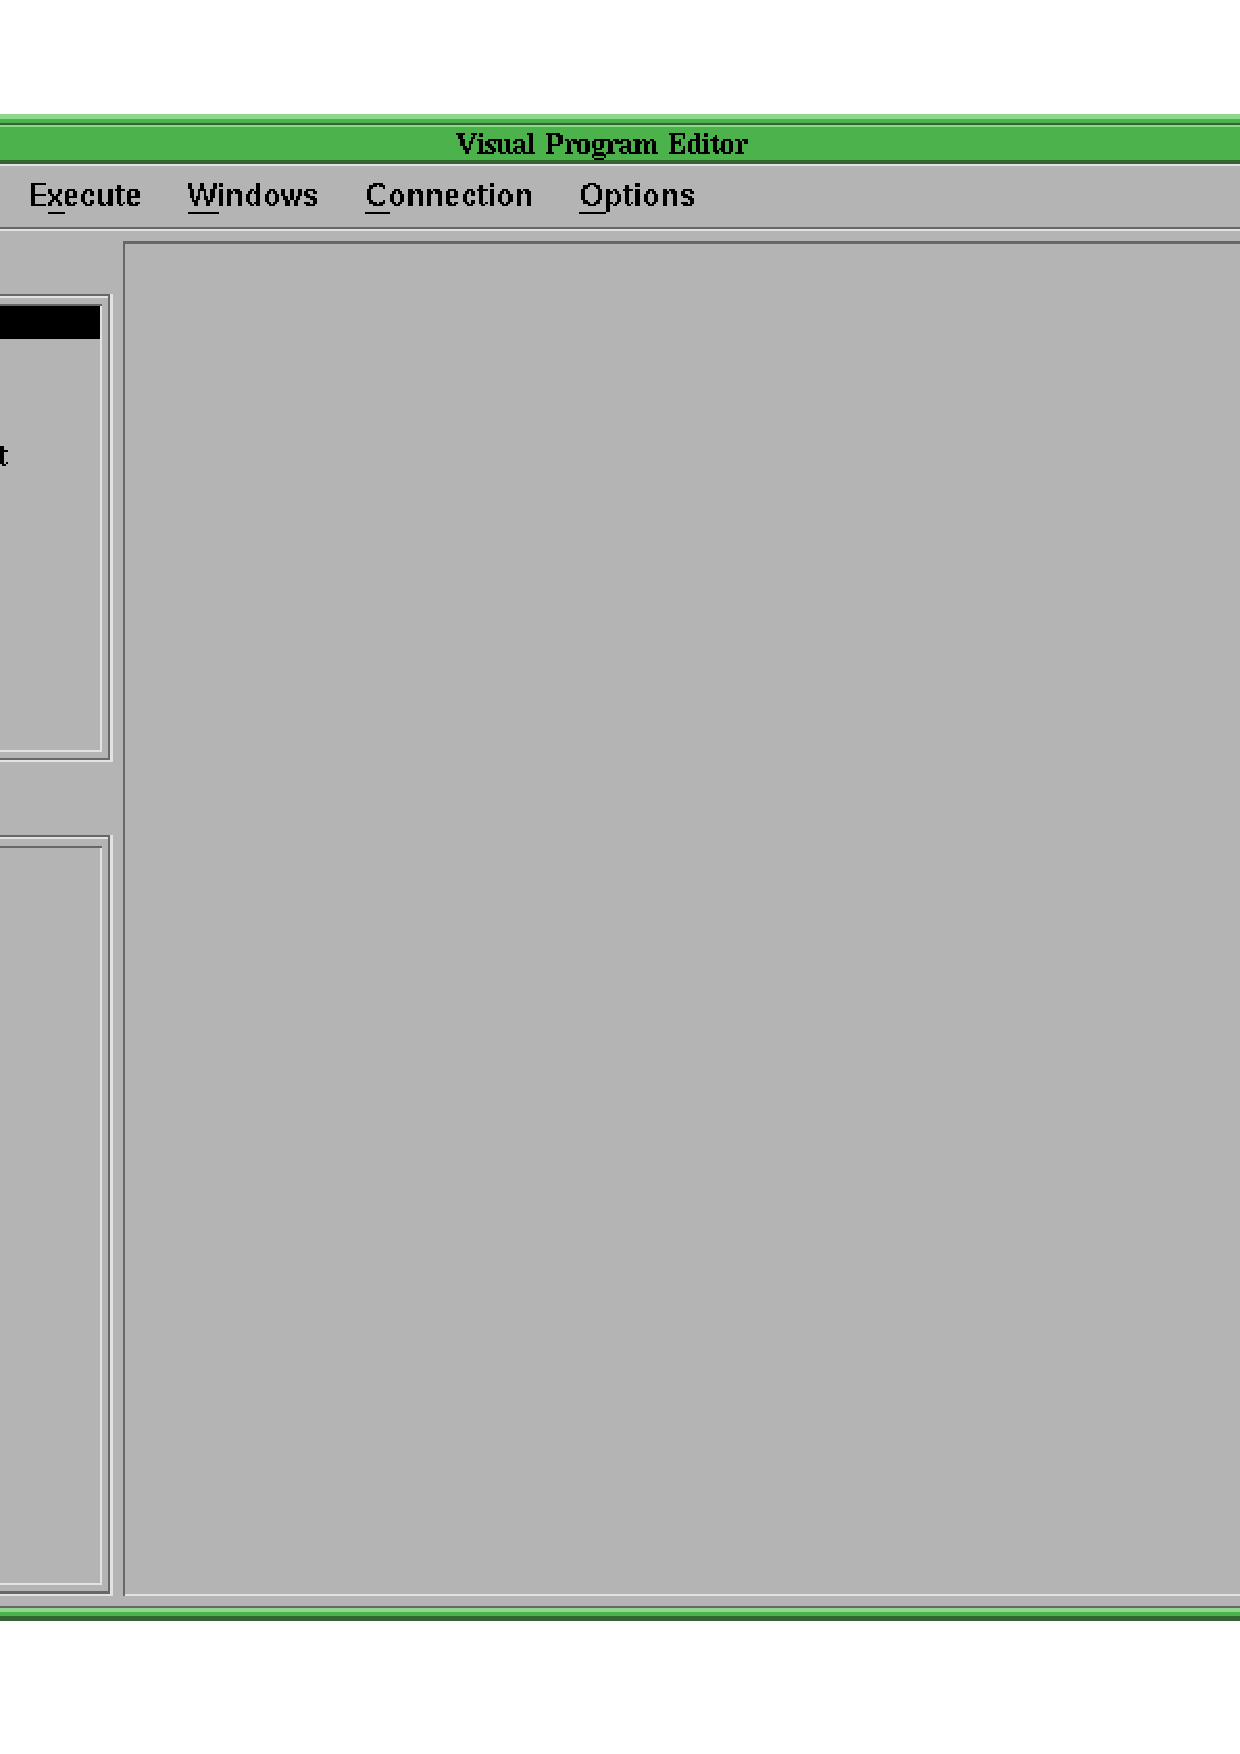
\includegraphics[width=450pt]{sc2_vpe}
  \end{center}

  \caption[The main window for the Visual Program Editor.]{The main
   window for the Visual Program Editor.}

  \end{figure}

  \item Figure~\ref{VPE} shows the main window for the Visual Program
   Editor (VPE). You will use it to construct DX networks which in turn
   will generate visualisations.

  \begin{itemize}

    \item The large blank area is the canvas where the network will be
     constructed.

    \item A DX network consists of modules, represented by icons, each
     performing some function. The collection of modules is divided
     into categories of similar modules. On the left hand side of the
     VPE are two boxes containing lists of items. The top box, labelled
     `Categories:', lists all the different categories of modules. The
     current category is highlighted (it is `Annotation' in
     Figure~\ref{VPE}). The lower box, labelled `Annotation Tools',
     shows all the modules in the current category.

     To choose another category simply click on the category required.
     The new category will be highlighted and both the label and the
     contents of the lower box will be changed to reflect the new
     choice.

  \end{itemize}

  \item To place a module on the canvas (for subsequent inclusion in a
   network) proceed as follows:

  \begin{enumerate}

    \item select the appropriate category, so that the required module
     appears in the lower box,

    \item click on the required module in the lower box, and it will be
     highlighted,

    \item move the cursor to the desired position in the canvas and
     click again. The module will appear as a rectangular icon (see,
     for example, Figure~\ref{SIMPLE}).

  \end{enumerate}

  \item If you want to move a module to another position in the canvas
   (for example, because you have inadvertently put it in the wrong
   place):

  \begin{enumerate}

    \item click in the body of the module and hold down the leftmost
     mouse button,

    \item move the cursor to the new position (continuing to hold down
     the mouse button),

    \item release the mouse button.

  \end{enumerate}

  \item To delete a module from the canvas:

  \begin{enumerate}

    \item click in the body of the module. It should appear highlighted,
     with a white bar above and below it,

    \item choose the `Delete' option from the `Edit' menu and the module
     should disappear from the canvas.

  \end{enumerate}

  \item The icons representing modules usually have tabs projecting
   from their top and bottom sides.

  \begin{itemize}

    \item The tabs along the top represent inputs to the module.

    \item The tabs for mandatory inputs are coloured a brighter shade
     of green; optional (or defaulted) inputs are the same colour as
     the body of the icon.

    \item The tabs along the bottom represent outputs.

  \end{itemize}

   In DX data can only flow from an output tab to an input tab. An
   input tab can only be fed by one output tab. However, an output tab
   can feed an arbitrary number of input tabs.

  \item To connect an output to an input:

  \begin{enumerate}

    \item click on the output tab and hold the leftmost mouse button
     down,

    \item move the cursor to the input tab, continuing to hold the
     mouse button down,

    \item release the mouse button.

  \end{enumerate}

   A line should be drawn from the output to the input tab (not all
   input and output types are compatible; if the tabs are not compatible
   DX will not connect them with a line).

  \item To remove the connection between an input and output:

  \begin{enumerate}

    \item click on the \textit{input}\, tab and hold down the leftmost
     mouse button,

    \item move the cursor to a blank portion of the canvas,

    \item release the mouse button, and the connection will vanish.

  \end{enumerate}

  \item At this juncture, practice positioning modules on the canvas,
   deleting them and connecting them, until you have got the hang of it.

  \item Values for input tabs can be specified as defaults as an
   alternative to supplying a value from an output tab. This mechanism
   is often used to specify the name of the data file which a network
   is to operate on, as well as to supply other values needed by a
   network. The procedure is as follows:

  \begin{enumerate}

    \item double-click on the module for which an input value is to be set,

    \item a new window, called the configuration window, should appear,
     showing the commonly used inputs for the module. Figure~\ref{IMPORT}
     shows this window for the `Import' module,

    \begin{figure}[htbp]

    \begin{center}
    \leavevmode
    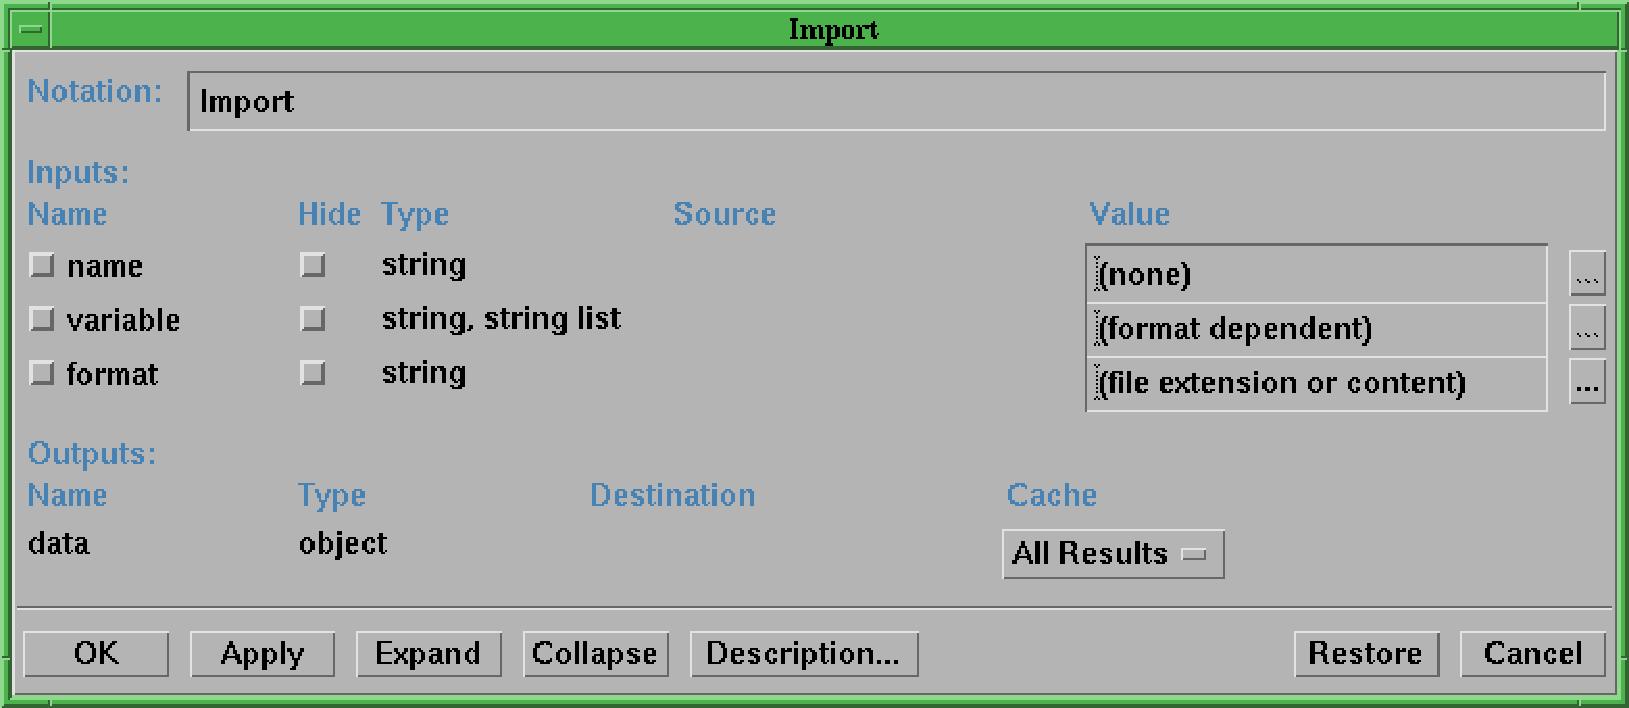
\includegraphics[width=450pt]{sc2_import}
    \end{center}

    \caption[Window for the `Import' module.]{Window for the `Import'
     module.\label{IMPORT} }


    \end{figure}

    \item each line of the `Inputs' section of the window corresponds
     to a separate input; their names are listed on the right hand
     side. For module `Import' the inputs are `name', `variable' and
     `format',

    \item click on the `Value' box for the chosen input,

    \item hold down the leftmost mouse button and drag it over the
     existing value, so that the existing value is highlighted,

    \item type in the new value,

    \item hit return (\textit{do not forget this step}),

    \item after you have hit return DX will display the value that you
     have entered, inside the box, in double quotation marks,

    \item repeat the procedure until all the required inputs have been
     set, then click on the `OK' button.

  \end{enumerate}

   By default only the commonly used inputs for a module are shown. To
   show all the inputs (and outputs) click on the `Expand' button.

  \item Various on-line help information is available within DX. In
   particular, it is possible to get help on individual modules, which
   is useful both for finding out what a module does and for determining
   the input which it needs. To obtain help on a module proceed as
   follows:

  \begin{enumerate}

    \item click on the `Help' menu in the top right hand corner of
     the VPE (see Figure~\ref{VPE}),

    \item choose menu-item `Context-Sensitive Help'; the mouse pointer
     will change to a `?',

    \item position the pointer over either the required module on the
     canvas or the name of the module in the list in the bottom left
     hand corner of the VPE, and click,

    \item another window containing a detailed description of the module
     will appear. Note that this information is formatted as hypertext,
     with links being indicated by a box drawn around the linked text.
     Simply click inside the box to follow the link,

    \item when you have finished perusing the text simply click on the
     `Close' button.

  \end{enumerate}

  \item Another useful trick is that if you position the pointer over
   an input or output tab and hold down the leftmost mouse button then
   while the button is depressed the name of the tab appears in the
   module icon. This feature is particularly convenient for identifying
   tabs.

  \item Now clear the canvas ready to start building a network: select
   option `New' from the `File' menu.

  \item Figure~\ref{SIMPLE} shows virtually the simplest possible DX
   network. You are now going to create this network.

  \begin{figure}[htbp]

  \begin{center}
  \leavevmode
  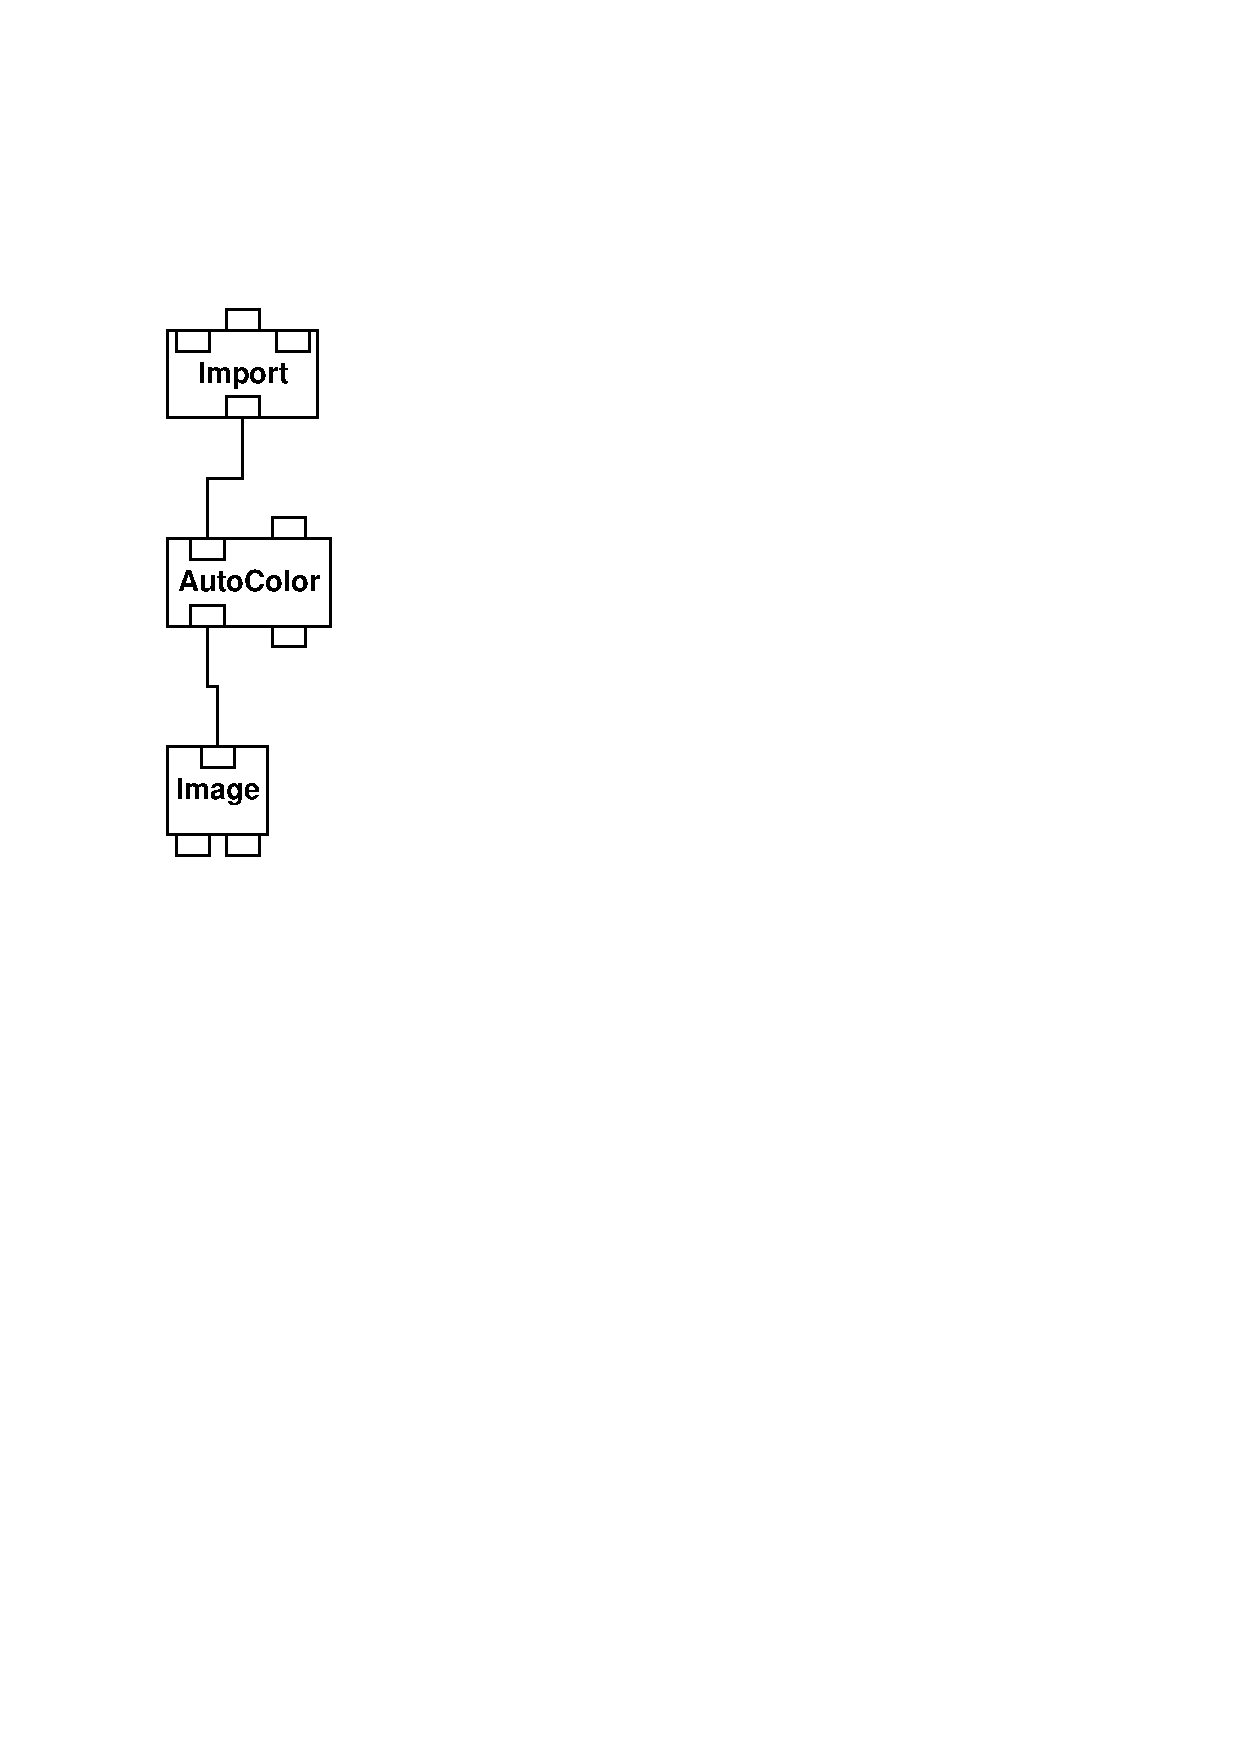
\includegraphics[width=139pt]{sc2_simple}
  \end{center}

  \caption[A simple network.]{A simple network. \label{SIMPLE} }

  \end{figure}

   There are two ways to create the network. The first is to find the
   three modules, position them on the canvas and join them as shown.
   The second is to read in a prepared copy of the network from a file.
   For the second option proceed as follows.

  \begin{enumerate}

    \item Select `Open Program' from the `File' menu.

    \item The `Open\ldots' window appears, as shown in
     Figure~\ref{OPEN}. You will use this window to specify the network
     file.

    \newpage
    \begin{figure}[htbp]

    \begin{center}
    \leavevmode
    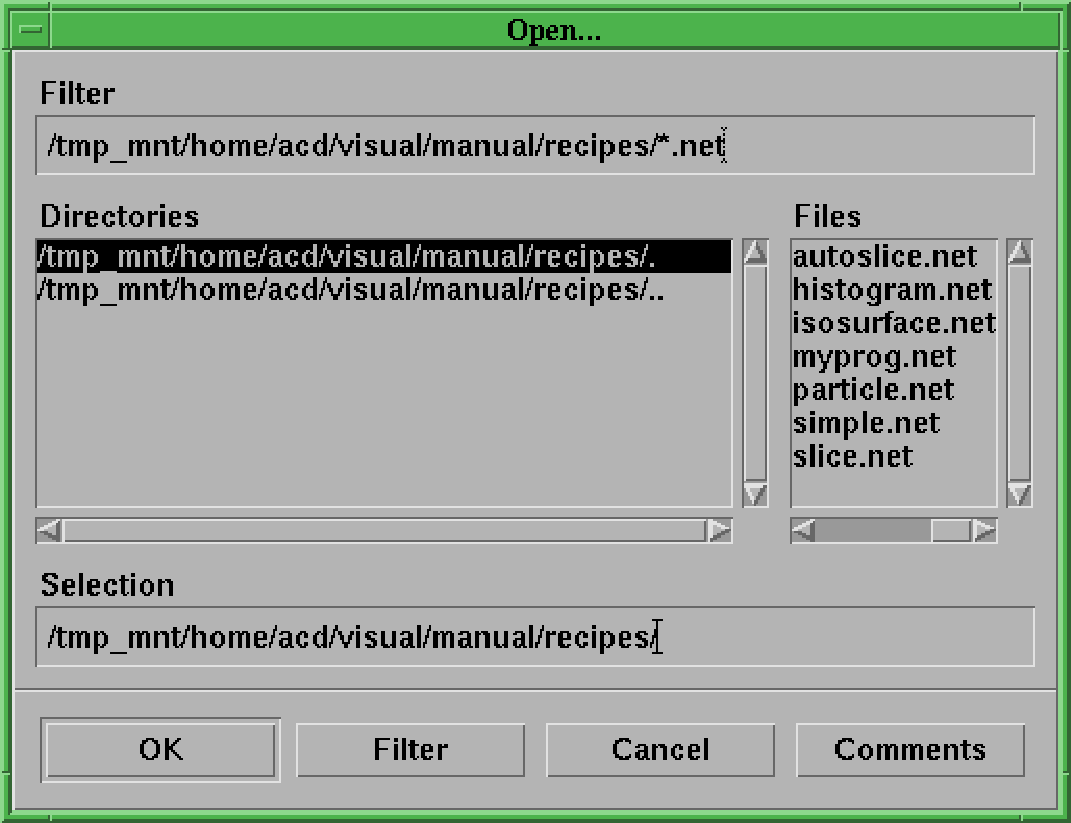
\includegraphics[width=450pt]{sc2_open}
    \end{center}

    \caption[The `Open\ldots' window.]{The `Open\ldots' window.
    \label{OPEN} }


    \end{figure}

    \item The `Filter' box at the top of the window controls the files
     available for selection. It contains a wild-card file expression
     and all the files which match the expression are available for
     selection. Click on this box and enter:

    \begin{quote}
     \texttt{\$STARLINK\_DIR/examples/sc2}
    \end{quote}

     A list of networks should appear in the `Files' box on the right
     hand side of the window. By convention DX networks have file type
     `\texttt{.net}'.

    \item Click on file `\texttt{simple.net}' in this box. The full file
     name and directory specification of the \texttt{simple} network should
     now appear in the `Selection' window.

    \item Click on the `OK' button. The `Open\ldots' window closes and
     the network is loaded onto the canvas.

  \end{enumerate}

   The network is now ready for use.

  \item The purpose of the three modules of the network is:

  \begin{description}

    \item[Import] read in the field to be displayed from an external
     file,

    \item[AutoColor] colour a field ready for display, so that a range
     of values in the field map to a range of colours,

    \item[Image] display a field. In this network `Image' will produce a
     volume rendering of a gridded dataset. However, it can accept
     various other sorts of input to produce different sorts of display.

  \end{description}

\end{enumerate}

\subsection{\label{RUNNET}Running a network}


Running a DX network to generate a visualisation comprises three stages:
specifying the input (particularly the file to be read), running the
network and examining the result. This example describes how to execute
the \texttt{simple} network loaded in the previous section. It will be used
to view an example data file, supplied with the cookbook, which contains
a data cube of a simple Gaussian. This data cube is a `field' in the
context of DX; see Section~\ref{OUTLINE} for an explanation of this
term.

\begin{enumerate}

  \item Double-click on the `Import' module; the configuration window
   shown in Figure~\ref{IMPORT} should appear.

  \begin{enumerate}

    \item Set input `name' to: \texttt{\$STARLINK\_DIR/examples/sc2/field.general}

     This file is the DX `header' file describing the data file.
     Files written by an external program and imported into DX are
     described by a separate header file. See Sections~\ref{IMP_GRID}
     and \ref{IMP_PART} for details. Note that it is the name of the
     header file, \textit{not}\, the data file, which is given here. If
     the header file is in your current directory then the directory
     specification can be omitted.

    \item Set input `variable' to: \texttt{Gaussian}

     This input specifies which field within the data file is to be
     read. In the current example the field is called `\texttt{Gaussian}'.
     Again see Sections~\ref{IMP_GRID} and \ref{IMP_PART} for details.

    \item Set input `format' to: \texttt{general}

     Here `\texttt{general}' means that the data file has been written by
     an external program and is described by a separate header file.
     The only other option which you are likely to encounter is `\texttt{dx}' for a native DX format file.

    \item When all the values have been set correctly simply click on
     the `OK' button.

  \end{enumerate}

  \item To run the network select `Execute Once' from the `Execute'
   menu.  The network will probably take a few minutes to run.

  \item After a few minutes a window containing the visualisation will
   appear. The options for this window allow you a great deal of choice
   in viewing the visualisation. The following couple of hints might be
   useful.

  \begin{itemize}

    \item DX is a bit lackadaisical about resetting the limits of the
     plot when a new visualisation is generated. If your visualisation
     does not neatly fill the plotting window (it may be either too big
     or too small) select the `Reset' option from the `Options' menu.

    \item By default DX generates a view perpendicular to one of the
     axes, which gives an unnaturally `flat' appearance to the image.
     For a better perspective view select the `View Control' option
     from the `Options' menu. The `View Control' window appears. Set the
     `Set View' toggle to `Diagonal' or one of the `Off\ldots' options.

  \end{itemize}

\end{enumerate}


\newpage
\section{\xlabel{IMP_GRID}\label{IMP_GRID}Importing Gridded Data}


It is usually possible to input a file written by some other program
into DX. The procedure is simply to create a file which describes the
contents of the data file to DX. This description file is called a
`header file' and is simply a text file created with an editor.

As an example this recipe shows how to import a formatted text file
containing two data cubes. One data cube is a simple Gaussian field,
the other is a Gaussian superimposed on a sloping background. Note that
though the values are calculated using Fortran double precision
variables they are written out as floating point numbers. DX interprets the
ensuing file as containing single precision values. Each data cube is
represented as a single DX field (see Section~\ref{OUTLINE}).
The program to generate the data file is listed in Figure~\ref{FIELD.F}.

\begin{enumerate}

  \item The DX header file for this data file is shown in
   Figure~\ref{FIELD.GENERAL}. These header files have file type
   `\texttt{.general}'. Thus the present example is called `\texttt{field.general}'.

  \begin{figure}[htbp]

\begin{quote}
\begin{terminalv}
file=field.lis
format=text
grid=50x50x50
majority=row
interleaving=field
field=Gaussian, Sloping
structure=scalar, scalar
type=float, float
dependency=positions, positions
\end{terminalv}
\end{quote}

  \caption[Header file for gridded data.]{Header file for gridded data.
  \label{FIELD.GENERAL} }

  \end{figure}

  \item Each line of the header file consists of a keyword followed by
   one or more values. The purpose of the various keywords are as
   follows.

  \begin{description}

    \item[file] is the name of the data file. If the file name is not
     preceded by a directory specification then it is assumed to be in
     the same directory as the header file.

    \item[format] is the format of the file; the current example is
     a formatted file rather than a binary file.

    \item[grid] is the size of the grid of data. In the present case
     both data cubes comprise grids with fifty elements in each side.

    \item[majority] specifies the organisation of multi-dimensional
     arrays. `Column' majority means that the first dimension varies
     fastest (as in Fortran); `row' majority means that the last
     dimension varies fastest (as in C).

    \item[interleaving] specifies how the data for the two fields are
     interleaved within the file. DX permits various possibilities.
     For example, all the values for the first field could occur
     first, followed by all the values for the second field. In the
     present case the data for the two fields are more closely
     intertwined. Each record in the file contains a value for a
     position in the first field and a value for the corresponding
     position in the second field (see Figures~\ref{GRID_DATA} and
     \ref{FIELD.F}). `\texttt{interleaving=field}' specifies this
     sort of interleaving.

    \begin{figure}[htbp]

    \begin{center}
    \begin{tabular}{l}
     \texttt{0.15655673~~~~~~~~0.25655673} \\
     \texttt{0.16572675~~~~~~~~0.26572675}  \\
     \texttt{0.17514088~~~~~~~~0.27514088}  \\
     \texttt{0.18476781~~~~~~~~0.28476781}  \\
     \texttt{0.19457102~~~~~~~~0.29457102}  \\
     \texttt{0.20450866~~~~~~~~0.30450866}  \\
     \texttt{~~~~~$\vdots$~~~~~~~~~~~~~~~~~$\vdots$}  \\
    \end{tabular}
    \end{center}

    \begin{quote}
    \caption[File \texttt{field.lis}.]{The first few records of file \texttt{field.lis} (written by program \texttt{field.f},
     Figure~\ref{FIELD.F}). The first column is values for the simple
     Gaussian data cube, the second column values for the Gaussian
     superimposed on a sloping background. \label{GRID_DATA} }
    \end{quote}

    \end{figure}

    \item[field] specifies names for the fields in the file. Here
     they are called `Gaussian' (the simple Gaussian data cube) and
     `Sloping' (the Gaussian superimposed on a sloping background).
     Note the use of a comma to separate the two names.

    \item[structure] specifies the structure of the two fields in the
     file. In the current example both the fields are simple scalars.

    \item[type] specifies the data types of the two fields. In the
     current example both fields are single precision real numbers.

    \item[dependency] denotes whether the data are position or
     connection dependent. See Section~\ref{POSCONDEP} for an
     explanation of these two cases. Here both fields are position
     dependent (which is probably the more common case in astronomy).

  \end{description}

   A full description of all the possible keywords is given in
   Section~4.3 \textit{Header File Syntax: Keyword Statements}\, of the
   IBM \textit{QuickStart Guide}\cite{QUICKS}.

  \item Once a suitable description file has been been created the data
   can be imported into DX by including the `Import' module in your
   network. Note that it is the name of the description file, \textit{not}\,
   the name of the data file which must be supplied to `Import'.

\end{enumerate}

\subsection{Variations}

\begin{enumerate}

  \item DX includes `Data Prompter', a windows-based application for
   interactively creating the header file for a data set. However, often
   it is no easier to use than creating the header file with an editor.
   Section 4.4 \textit{Data Prompter}, of the \textit{QuickStart
   Guide}\cite{QUICKS} gives details.

  \latex{\newpage}
  \item Unformatted binary files can also be imported using the same
   header file mechanism. The \texttt{format} keyword should be set to
   `\texttt{binary}'. Binary files written with a C program can be
   imported directly. However, unfortunately, binary files  written with
   a Fortran program contain record-control bytes which must be
   removed prior to importing the file. The Starlink extensions to DX
   include \texttt{SXUnfort} for this purpose; see
   \xref{SUN/203}{sun203}{}\cite{SUN203} for details. Of course, an
   unformatted file written on a Digital alpha will differ from the
   corresponding file written on a Sun because of the different byte
   order of the machines. It is possible to input an unformatted file
   written on a Sun into DX running on a Digital alpha, or vice versa, by
   using the `\texttt{msb}' and `\texttt{lsb}' modifiers to the \texttt{format}
   keyword\footnote{Strictly speaking it should be possible to input any
   unformatted file written in IEEE floating point format, irrespective
   of the type of machine that it was written on. Note, however, that
   Digital VAXen and IBM mainframes do not use IEEE floating point format.}.
   See Section~4.3 \textit{Header File Syntax: Keyword Statements}\, of the
   IBM \textit{QuickStart Guide}\cite{QUICKS} for details.

  \item It is also possible to import files in the Starlink NDF format
   (and other common astronomical formats, such as FITS images or Figaro
   DST files). Again see \xref{SUN/203}{sun203}{}\cite{SUN203} for details.

\end{enumerate}

\begin{figure}[htbp]

\begin{terminalv}
      PROGRAM FIELD
      IMPLICIT NONE
*    Generate two data cubes.  One contains a Gaussian function, the
*    other a Gaussian on a sloping background.
*    A C Davenhall (Edinburgh), 3/12/95.
      DOUBLE PRECISION
     :  XCEN,   ! X Centre of distribution.
     :  YCEN,   ! Y   "    "       "      .
     :  ZCEN,   ! Z   "    "       "      .
     :  A,      ! Scale factor.
     :  B,      ! Exponential scale factor.
     :  C       ! Background slope.
      PARAMETER
     : (XCEN = 2.5D1,  YCEN = 2.5D1,  ZCEN = 2.5D1,
     :  A = 1.0D1,     B = 1.0D1,     C = 1.0D-1)
      DOUBLE PRECISION
     :  DIST,   ! Distance of point from centre.
     :  VALUE1, ! Value of Gaussian function at the point.
     :  VALUE2  ! Value of Gaussian on sloping background at the point.
      INTEGER
     :  I, J, K ! Loop indices.

      OPEN(UNIT=10, FILE='field.lis', STATUS='NEW')

      DO I = 1, 50
         DO J = 1, 50
            DO K = 1, 50
               DIST = SQRT( ((REAL(I) - XCEN)**2) +
     :           ((REAL(J) - YCEN)**2) +
     :           ((REAL(K) - ZCEN)**2) )

               VALUE1 = A*EXP(-DIST / B)
               VALUE2 = VALUE1 + (C * REAL(I))

               WRITE(10, '(1X, 0PF16.8, 2X, 0PF16.8)' ) VALUE1, VALUE2
            END DO
         END DO
      END DO

      CLOSE(UNIT=10)

      END
\end{terminalv}

\caption[Program \texttt{field.f} to write gridded data.]{Program \texttt{field.f} to write gridded data. \label{FIELD.F} }

\end{figure}


\newpage
\section{\xlabel{IMP_PART}\label{IMP_PART}Importing Particle Data}


It is usually possible to input a file written by some other program
into DX. The procedure is simply to create a file which describes the
contents of the data file to DX. This description file is called a
`header file' and is simply a text file created with an editor.

As an example this recipe shows how to input a formatted text file
containing particle (or catalogue) data. The positions of the particles
trace out a three-dimensional cone. The data are represented as a
single DX field (see Section~\ref{OUTLINE}). For simplicity the file
contains only this single field. However, it is possible to have
particle datasets containing several fields, similar to the gridded
data in Section~\ref{IMP_GRID}. The program to generate the data is listed
in Figure~\ref{PARTICLE.F}.

\begin{enumerate}

  \item The DX header file for this data file is shown in
   Figure~\ref{PARTICLE.GENERAL}. These header files have file type
   `\texttt{.general}'. Thus the present example is called `\texttt{particle.general}'.

  \begin{figure}[htbp]

  \begin{quote}
\begin{terminalv}
file=particle.lis
points=10000
format=text
field=locations, Intensity
structure=3-vector, scalar
interleaving=field
\end{terminalv}
  \end{quote}

  \caption[Header file for particle data.]{Header file for particle
   data. \label{PARTICLE.GENERAL} }

  \end{figure}

  \item Each line of the header file consists of a keyword followed by
   one or more values. The purpose of the various keywords are as follows.

  \begin{description}

    \item[file] is the name of the data file. If the file name is not
     preceded by a directory specification then it is assumed to be in
     the same directory as the header file.

    \item[points] is the number of particles (or points) in the data
     set.

    \item[format] is the format of the file; the current example is
     a formatted file rather than a binary file.

    \item[field] specifies names for the the individual fields (or columns) in
     the data file. In the present case the first three columns,
     containing the positions are collectively called `locations' and
     the final column is called `Intensity'. Note the use of a comma to
     separate the two names.

    \item[structure] specifies the structure of each field in the file.
     In the present case the first three columns are grouped into a
     three-element vector containing the positions and the fourth
     column is treated as a scalar dependent variable.

    \item[interleaving] specifies how the various data items within
     the file are intertwined. In the present case each record in the
     file contains the position and data value for a single particle
     (see Figure~\ref{PARTICLE.F}). `\texttt{interleaving=field}'
     specifies this sort of interleaving.

  \end{description}

   A full description of all the possible keywords is given in
   Section~4.3 \textit{Header File Syntax: Keyword Statements}\, of the
   IBM \textit{QuickStart Guide}\cite{QUICKS}.

  \newpage
  \item Once a suitable description file has been been created the data
   can be imported into DX by including the `Import' module in your
   network. Note that it is the name of the description file, \textit{not}\,
   the name of the data file which must be supplied to `Import'.

\end{enumerate}

\subsection{Variations}

See the notes for variations of \textit{Importing Gridded Data},
Section~\ref{IMP_GRID}, above.

\begin{figure}[htbp]

\begin{terminalv}
      PROGRAM PARTICLE
      IMPLICIT NONE
*    Generate a particle dataset, with the individual particles tracing
*    out positions on a cone.  The dependent variable varies
*    (indirectly) with the Z distance.
*    A C Davenhall (Edinburgh), 4/12/95.
      REAL
     :  DR,      ! Increment in radius.
     :  DTHETA,  !     "     "  theta.
     :  DZ,      !     "     "  z.
     :  PI       ! Pi.
      PARAMETER
     : (DR = 1.0E-1,  DTHETA = 1.0E-2,
     :  DZ = 1.0E-1,  PI = 3.1415927E0)
      REAL
     :  R,       ! Radius.
     :  THETA,   ! Theta.
     :  X,       ! X coordinate.
     :  Y,       ! Y     "     .
     :  Z,       ! Z     "     .
     :  VALUE    ! Value of the point.
      INTEGER
     :  I, J, K  ! Loop indices.

      OPEN(UNIT=10, FILE='particle.lis', STATUS='NEW')

      DO I = 1, 10000
         R = REAL(I) * DR
         THETA = REAL(I) * DTHETA
         THETA = MOD(THETA, 2*PI)
         X = R * COS(THETA)
         Y = R * SIN(THETA)
         Z = REAL(I) * DZ

         VALUE = SIN(MOD( REAL(I)/5.0E3, 2*PI) )

         WRITE(10, '(0PE12.4, 1X, 0PE12.4, 1X, 0PE12.4, 1X, 0PE12.4)' )
     :     X, Y, Z, VALUE
      END DO

      CLOSE(UNIT=10)

      END
\end{terminalv}

\caption[Program \texttt{particle.f} to write particle data.]{Program \texttt{particle.f} to write particle data. \label{PARTICLE.F} }

\end{figure}


\newpage
\section{\xlabel{HISTNET}\label{HISTNET}Displaying a Histogram}


\begin{tabular}{ll}
file:               & \texttt{histogram.net} \\
example data files: & \texttt{field.general}, \texttt{particle.general} \\
\end{tabular}

This network plots a histogram of the data values in a data set (strictly
speaking in a DX field; see Section~\ref{OUTLINE}). It also displays the
median, minimum and maximum values in the data. It will work on
$n$-dimensional gridded data and $n$-dimensional particle data. It can be
used for preliminary investigation of a dataset about which you have no
prior knowledge, in order to determine the range and distribution of
values which it contains.

\subsection{Use}

The network is shown in Figure~\ref{HISTNETF}.

\begin{figure}[htbp]

\begin{center}
\leavevmode
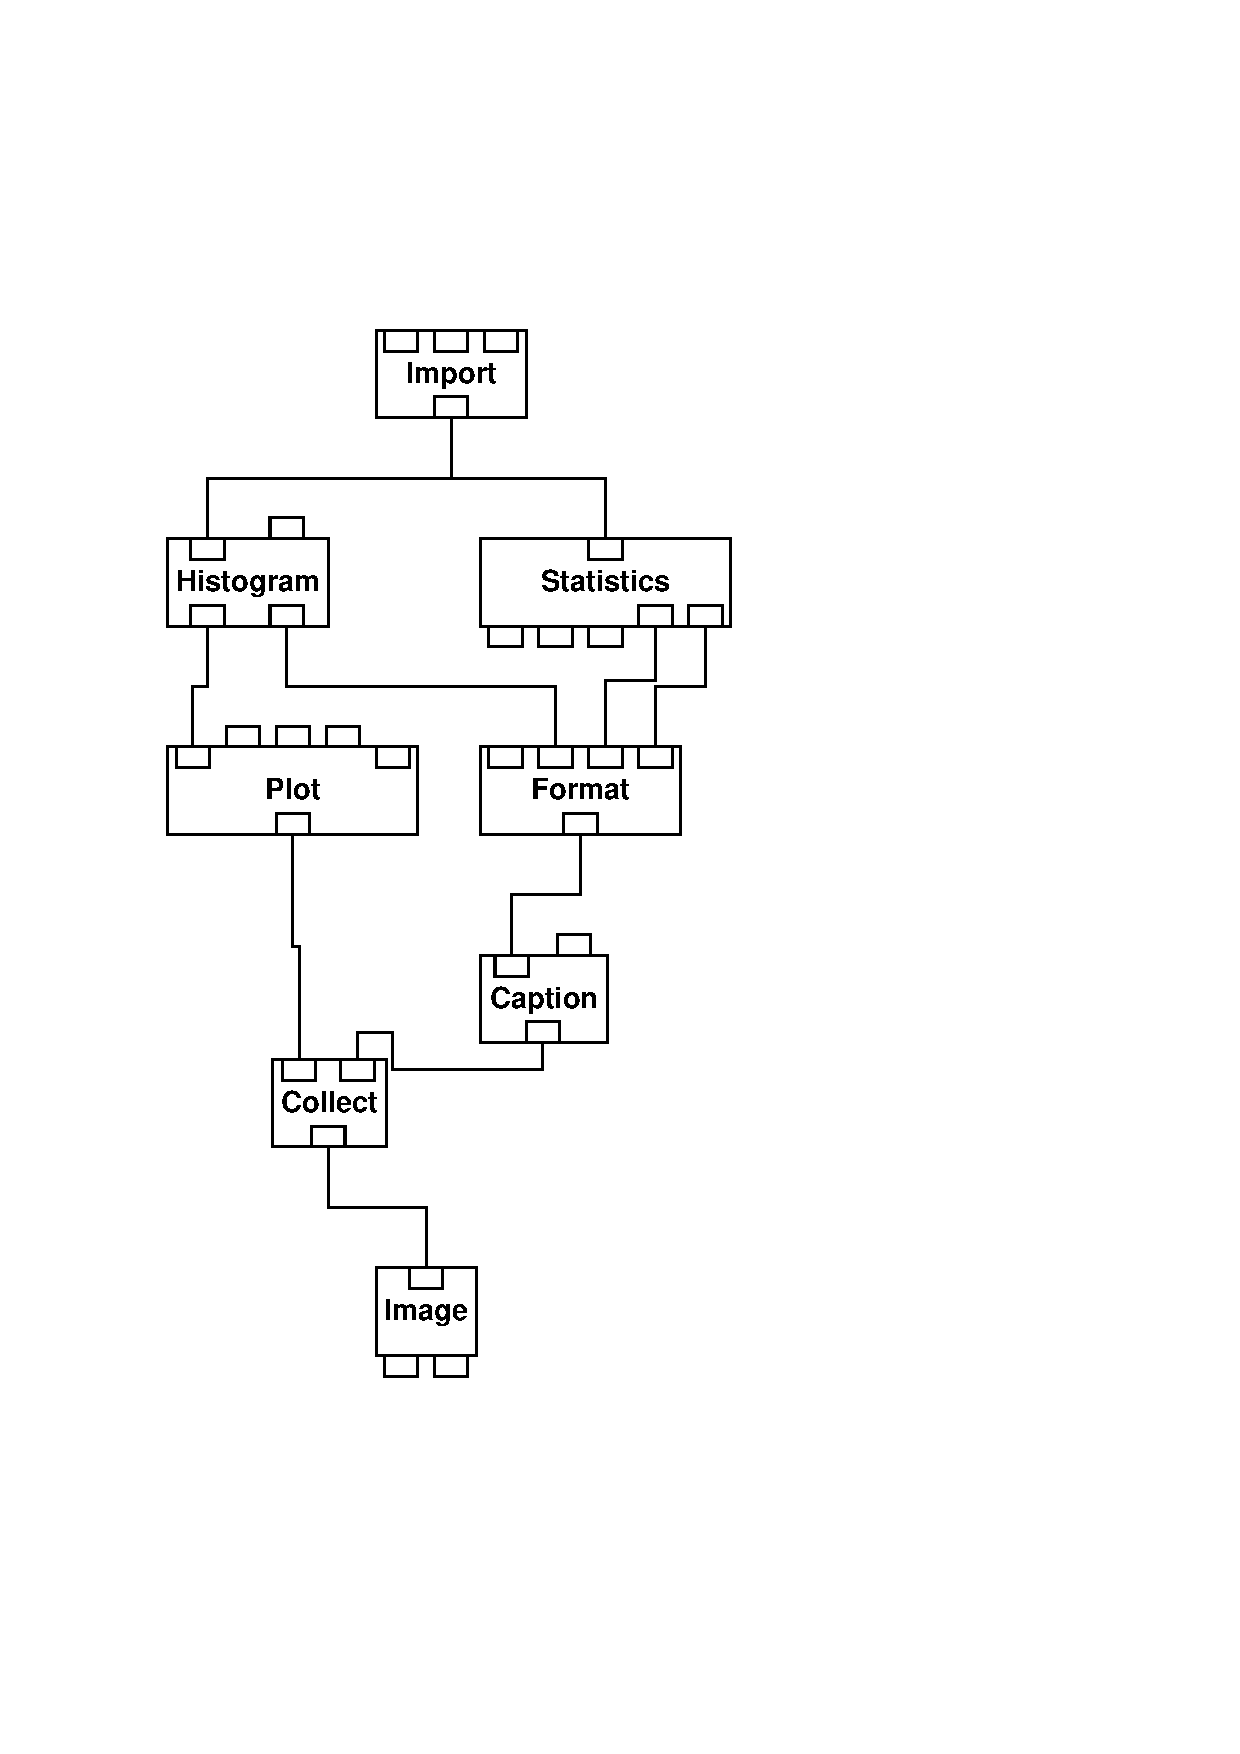
\includegraphics[width=371pt]{sc2_histogram}
\end{center}

\caption[Network to display a histogram.]{Network to display a histogram.
\label{HISTNETF} }

\end{figure}

\begin{itemize}

  \item To specify the data cube to be read double-click on the `Import'
   module and follow the instructions in Section~\ref{RUNNET}.

  \item By default the histogram will contain 100 bins (unless the data
   are of data type byte, in which case it will contain 256 bins). To
   specify the number of bins double-click on the `Histogram' module
   and set the input `bins' to the value required.

  \item By default the network generates a histogram spanning the
   entire range of values in the data set. You may need to control
   the range of values histogramed (for example, to prevent a few
   rogue values from dominating the $x$ range of the plot). The
   simplest way to control the $x$ range is to set the `min' and `max'
   inputs of the `Histogram' module.

\end{itemize}

\subsection{Notes}

The histogram is generated by module `Histogram' and turned into a graph
by module `Plot'. The minimum and maximum values in the data are
calculated by `Statistics'. `Format' and `Caption' assemble the median,
minimum and maximum into a text string and `Collect' combines the string
with the graph.

\subsection{Alternatives}

If your data are in Starlink NDF format then an alternative way to
generate a histogram is to use command \xref{\texttt{HIST}}{sun86}{HIST} in
Figaro (see \xref{SUN/86}{sun86}{}\cite{SUN86}).  This option will work
for $n$-dimensional gridded data.


\newpage
\section{\xlabel{SLICNET}\label{SLICNET}Displaying a Slice}


\begin{tabular}{ll}
file:              & \texttt{slice.net}     \\
example data file: & \texttt{field.general} \\
\end{tabular}

This network displays a two-dimensional slice through a data cube,
parallel to two of the axes. The slice is plotted as a false colour
array shown in its correct relative position inside a set of axes
representing the edges of the data cube. Note that the colour table for
converting data values into displayed colours is derived from the range
of values in the entire data cube, not just the slice being plotted,
in order to facilitate the comparison of several slices.

\subsection{Use}

The network is shown in Figure~\ref{SLICNETF}.

\begin{figure}[htbp]

\begin{center}
\leavevmode
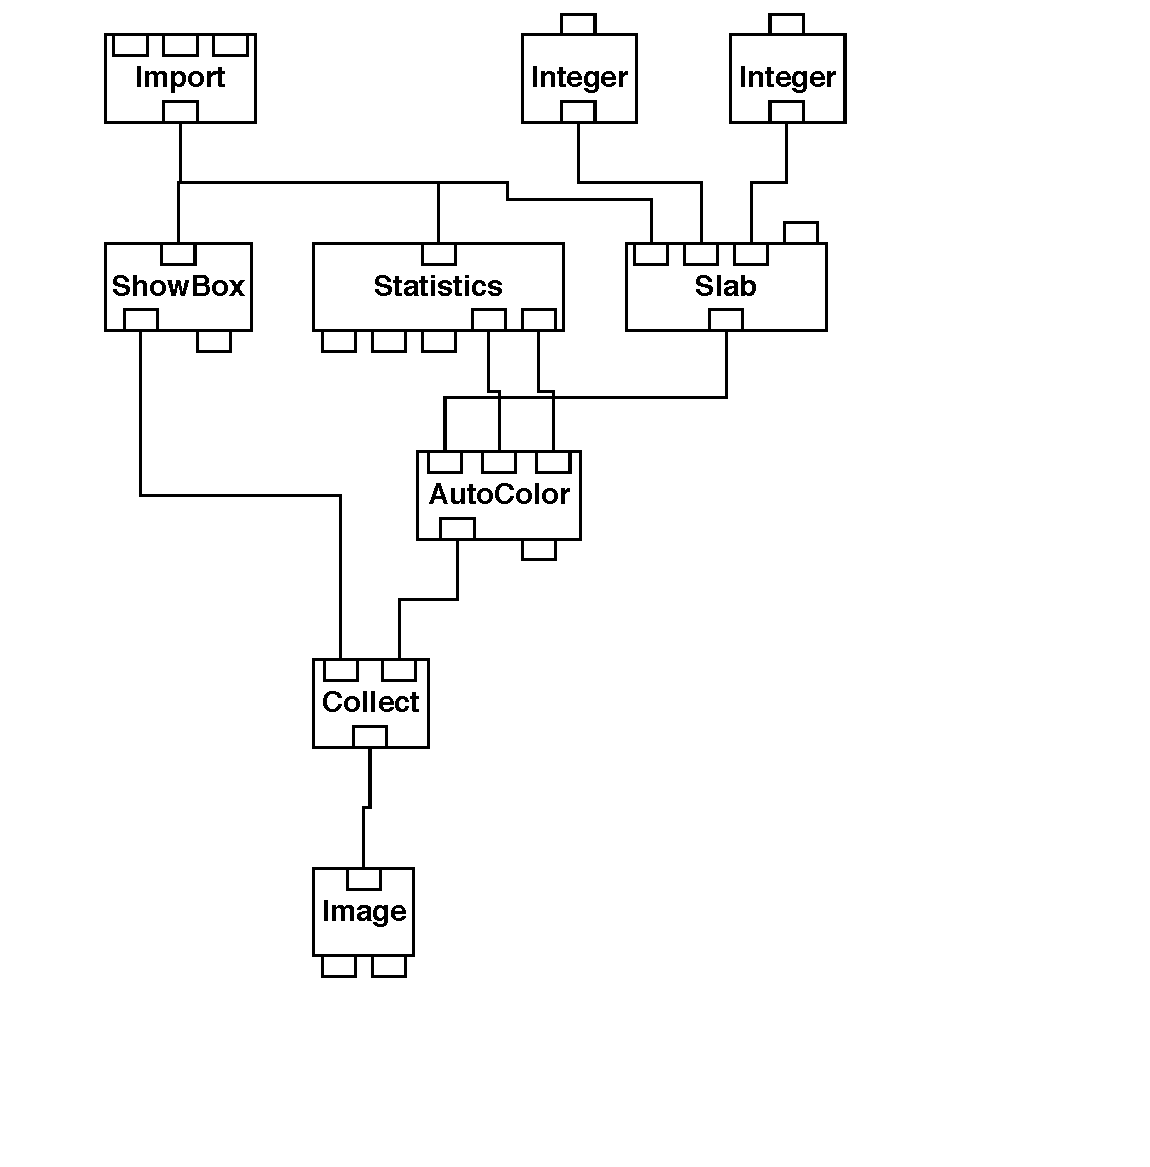
\includegraphics[width=553pt]{sc2_slice}
\end{center}

\caption[Network to display a slice through a data cube.]{Network to
display a slice through a data cube. \label{SLICNETF} }

\end{figure}

\begin{itemize}

  \item To specify the data cube to be read double-click on the `Import'
   module and follow the instructions in Section~\ref{RUNNET}.

  \item To specify the axis to which the slice is perpendicular
   double-click on the left-hand of the two `Integer' modules at the
   top of the network. The permitted values are 0, 1 and 2 for the
   $x, y$\, and  $z$\, axes respectively.

  \item To specify the slice which is to be extracted double-click on
   the right-hand of the two `Integer' modules at the top of the
   network. For a cube with $n$\, elements along the chosen axis the
   permitted values are 0 to $n-1$.

\end{itemize}

\subsection{Notes}

Module `ShowBox' extracts the bounding box of the data cube. `Slab'
extracts the specified slice. `Statistics' finds the minimum and
maximum values in the cube; they are used by `AutoColor' to generate
a false colour image of the extracted slice. `Collect' combines the
bounding box and extracted slice.

\subsection{Alternatives}

If your data are in Starlink NDF format then an alternative way to
plot a slice is to use command \xref{\texttt{DISPLAY}}{sun95}{DISPLAY} in KAPPA
(see \xref{SUN/95}{sun95}{}\cite{SUN95}).  You simply specify the required
slice, for example:

\begin{quote}
\texttt{DISPLAY~\textit{ndf\_file}(,,21)}
\end{quote}

plots the twenty-first slice in the third axis.

\newpage
\section{\xlabel{ASLICNET}Displaying a Sequence of Slices}


\begin{tabular}{ll}
file:              & \texttt{autoslice.net} \\
example data file: & \texttt{field.general} \\
\end{tabular}

This network is a modification of the network for displaying a
two-dimensional slice through a data cube parallel to two of the axes
(see Section~\ref{SLICNET}). Instead of displaying a single slice it
generates an animation showing successive slices `sweeping' through the
data cube. Note that, as before, the colour table for converting data
values into displayed colours is derived from the range of values in the
entire data cube, not just the current slice being plotted, in order to
facilitate visualisation as the current slice sweeps through the data
cube.

\subsection{Use}

The network is shown in Figure~\ref{ASLICNETF}.

\begin{figure}[htbp]

\begin{center}
\leavevmode
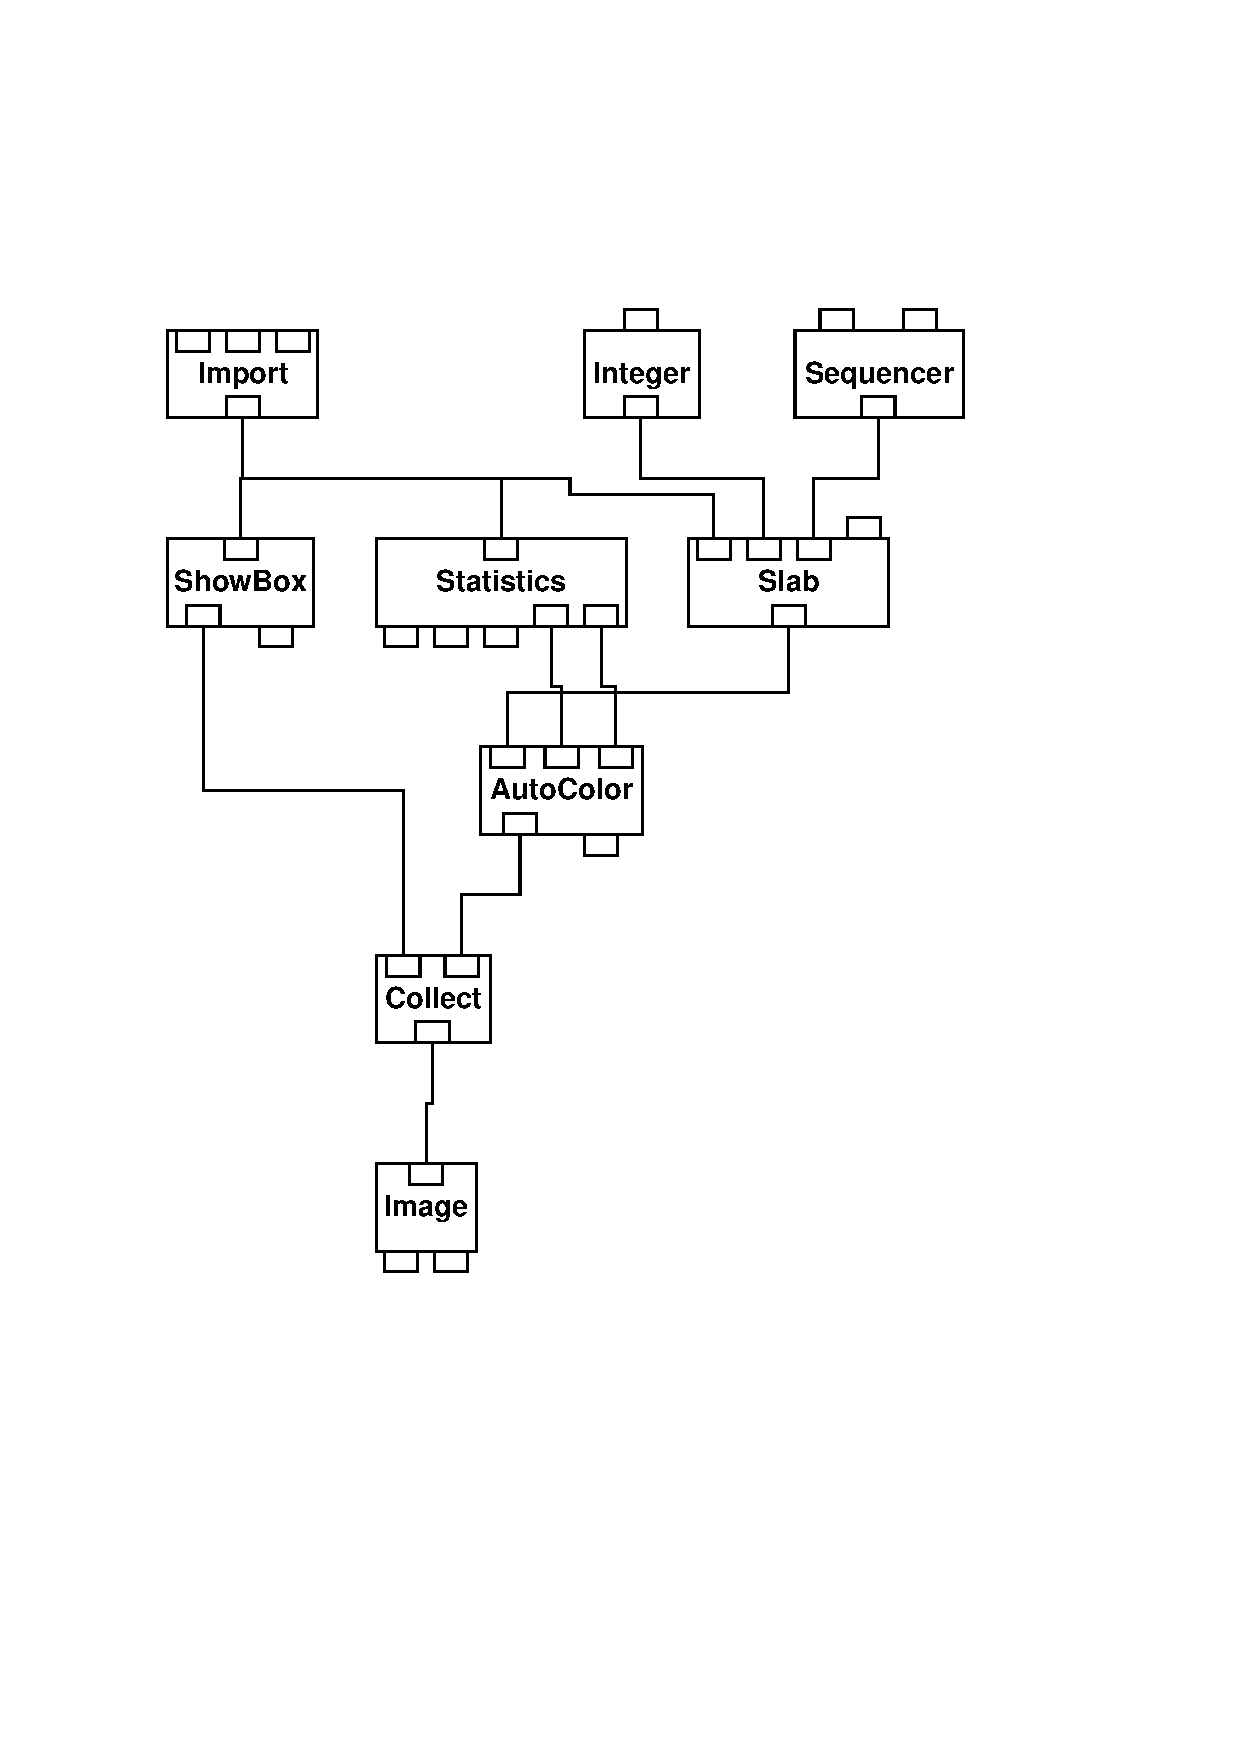
\includegraphics[width=553pt]{sc2_autoslice}
\end{center}

\caption[Network to display a sequence of slices in a data cube.]{Network
to display a sequence of slices in a data cube. \label{ASLICNETF} }

\end{figure}

\begin{itemize}

  \item To specify the data cube to be read double-click on the `Import'
   module and follow the instructions in Section~\ref{RUNNET}.

  \item To specify the axis to which the slice is perpendicular
   double-click on the `Integer' module at the top of the network. The
   permitted values are 0, 1 and 2 for the $x, y$\, and $z$\, axes
   respectively.

  \item To specify the range of slices to be shown double-click on the
   `Sequencer' module. A control panel with controls similar to (and
   corresponding functions to) the buttons on a cassette tape deck
   appears. Click on the ellipsis (`\ldots') button and a further window
   appears allowing you to specify the first and last slice to be
   extracted (and the increment between slices). For a cube with $n$\,
   elements along the chosen axis the permitted values are 0 to $n-1$.

   Finally, once you have chosen the required range, click on the play
   button (`$\triangleright$') in the original `Sequencer' window.

\end{itemize}

\subsection{Notes}

This network is identical to network \texttt{slice.net} for displaying
a single slice except that the right-hand of the two `Integer' modules
in \texttt{slice.net}, which specified the requested slice, has been
replaced with the `Sequencer' module.


\newpage
\section{\xlabel{ISOSURFNET}Displaying an Iso-surface}


\begin{tabular}{ll}
file:              & \texttt{isosurface.net} \\
example data file: & \texttt{field.general}  \\
\end{tabular}

This network displays an iso-surface\footnote{An iso-surface is the
analogue in three-dimensional gridded data of a single contour in
two-dimensional gridded data. That is, it is a surface defined by some
constant value of the dependent variable.} corresponding to some value in
a data cube. The colour of the iso-surface varies to mimic the effect
of light reflecting off the surface. The surface is plotted in its
correct relative position inside a set of axes representing the edges
of the data cube.

\subsection{Use}

The network is shown in Figure~\ref{ISOSURFNETF}.

\begin{figure}[htbp]

\begin{center}
\leavevmode
\includegraphics[width=271pt]{sc2_isosurface}
\end{center}

\caption[Network to display an iso-surface in a data cube.]{Network to
display an iso-surface in a data cube. \label{ISOSURFNETF} }

\end{figure}

\begin{itemize}

  \item To specify the data cube to be read double-click on the `Import'
   module and follow the instructions in Section~\ref{RUNNET}.

  \item To specify the value for the iso-surface double-click on the
   `Scalar' module at the top of the network and enter the required
   value.  If you have no knowledge of the range of values in the
   cube, and hence no idea of suitable value, use network \texttt{histogram.net} (see Section~\ref{HISTNET}) to find the minimum,
   maximum and distribution of values in the data.

\end{itemize}

\subsection{Notes}

Module `ShowBox' extracts the bounding box of the data cube.
`Isosurface' computes the iso-surface and `AutoColor' colours it.
`Collect' combines the bounding box and iso-surface.


\newpage
\section{\xlabel{PARTNET}Displaying Particle Data}


\begin{tabular}{ll}
file:              & \texttt{particle.net}     \\
example data file: & \texttt{particle.general} \\
\end{tabular}

This network displays three-dimensional particle data. Each point is
shown in its correct relative position inside a set of axes representing
a bounding box just enclosing the dataset. Note however that the
position of each point within the plot is necessarily ambiguous. Each
point is shown as a dot and coloured according to the data component of
the field.

\subsection{Use}

The network is shown in Figure~\ref{PARTNETF}.

\begin{itemize}

  \item To specify the data set to be read double-click on the `Import'
   module and follow the instructions in Section~\ref{RUNNET}.

\end{itemize}

\subsection{Notes}

Module `ShowBox' extracts the bounding box of the data set. `AutoColor'
generates a plot showing the positions of each point in the dataset and
colours each point according to the value of its data component.
`Collect' combines the bounding box and plot.

\begin{figure}[htbp]

\begin{center}
\leavevmode
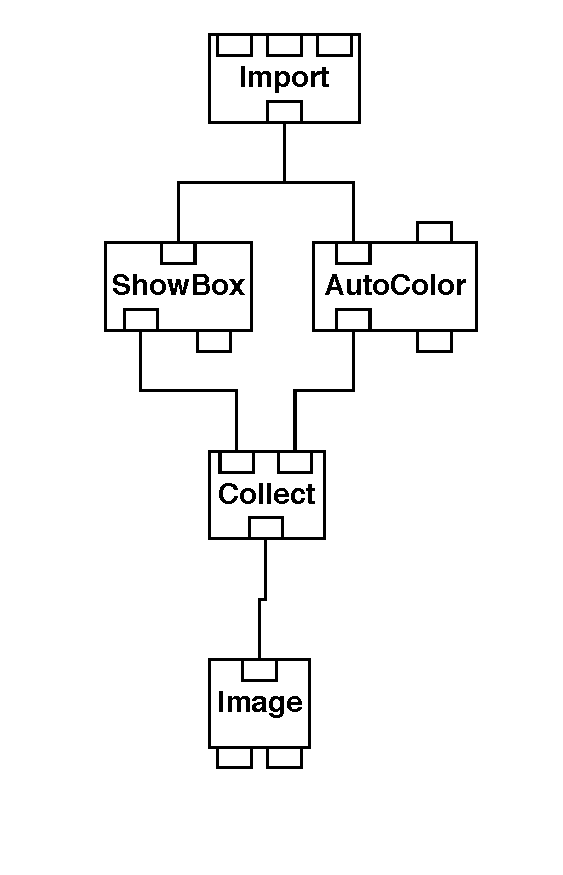
\includegraphics[width=271pt]{sc2_particle}
\end{center}

\caption[Network to display three-dimensional particle dataset.]{Network
to display three-dimensional particle dataset. \label{PARTNETF} }

\end{figure}


% - Part II -----------------------------------------------------------
\cleardoublepage

\part{Extended Recipes}

\section{\xlabel{INTRO_EXTEND}Introduction}

This section presents two extended recipes or case studies of using
DX.  Both recipes are concerned with importing and visualising
three-dimensional `cubes' of observational data.  In one case the data
were obtained with the James Clerk Maxwell Telescope (JCMT) in Hawaii
and in the other with the ROSAT X-ray astronomy satellite.  In both
cases two of the axes of the cube correspond to a grid of points on
the sky (in some projection) and the third axis to a spectrum in
frequency or energy.  The grids are regularly sampled in all three axes.

This section assumes that you are familiar with the basics of DX.  If
you are not familiar with DX then you should probably try some of
the simple networks in Part I.  At the very least you should be
follow the `Basic Use of DX' recipe (see Section~\ref{BASIC}).

\subsection{Copies of the recipe networks}

Like the simple networks in Part I, the networks and data files referred
to in this section can be found on Starlink systems in directory:

\begin{terminalv}
/star/examples/sc2
\end{terminalv}

and on non-Starlink systems in directory:
\begin{terminalv}
$STARLINK_DIR/examples/sc2
\end{terminalv}

The most convenient way to access these files is probably to copy them
into your current directory before attempting to read them or load
them into DX.  The examples in subsequent sections assume that copies
of the files are available in your current directory.


\newpage
\section{\xlabel{JCMT}\label{JCMT}JCMT Data Cube}

This recipe shows how to import and display a set of spectra observed
in the mm or sub-mm wavelength range of the electromagnetic spectrum
with a heterodyne receiver on the \htmladdnormallink{James Clerk Maxwell
Telescope}{http://www.eaobservatory.org/jcmt/} (JCMT) in Hawaii.
The example used here is an observation of emission from the C$^{18}$O ~
${\rm J} = 2 \rightarrow 1$ transition in L1689B, a dense core within
the molecular cloud Lynds Dark Nebula 1689.  The data cube comprises a
grid of 7 by 7 points on the sky, with a spectrum of 153 channels at each
position.  The example data are available as file \texttt{l1689b.sdf}.
JCMT heterodyne observations are usually reduced using the SPECX package
(see \xref{SUN/17}{sun17}{}\cite{SUN17}) and the example data are in the
native SPECX data format.  In SPECX terminology a collection of spectra
on a grid of points on the sky is a called a `map'.

\textit{The data for L1689B have kindly been made available in advance of
publication; they may not be published without the express, written
permission of the observers (see Section~\ref{ACK} for details).}

\begin{enumerate}

  \item The first stage to importing a SPECX map is to convert it to a
   simple data cube in the standard Starlink \xref{NDF}{sun33}{}
   format.  Application \texttt{specx2ndf} in the CONVERT package
   (see \xref{SUN/55}{sun55}{}\cite{SUN55}) performs this task.
   Proceed as follows.  First type:

\begin{terminalv}
% convert
\end{terminalv}

   to make the CONVERT applications available.  Then type:

\begin{terminalv}
% specx2ndf  l1689b  l1689bndf
\end{terminalv}

   Note that though the input SPECX map and output NDF are respectively
   held in files called \texttt{l1689b.sdf} and \texttt{l1689bndf.sdf}
   they are specified to application \texttt{specx2ndf} without the `\texttt{.sdf}' file type.

   When displaying SPECX maps it is conventional to represent the
   spectral axis as a series of radial velocities computed for the
   rest wavelength of the line being observed and corrected to a
   kinematical local standard of rest.  By default \texttt{specx2ndf}
   generates the spectral axis in this fashion and this is how it will
   be computed in the above example.  However, \texttt{specx2ndf} allows
   some flexibility in how the spectral axis is represented; see
   \xref{the appropriate section of SUN/55}{sun55}{SPECX2NDF} for
   details of the alternatives available.

  \item Once the SPECX map has been converted to a simple data cube in
   the NDF format it can be processed and displayed with a variety
   of standard Starlink applications, such as those in the image
   processing package KAPPA (see \xref{SUN/95}{sun95}{}\cite{SUN95}).
   For example, type:

\begin{terminalv}
% kappa
\end{terminalv}

   to make the KAPPA applications available.  Then type:

\begin{terminalv}
% hislist  l1689bndf
\end{terminalv}

   Again the file name is specified without the `\texttt{.sdf}' file type.
   This application lists the history information describing the
   processing which has been performed on the data.  The history
   information appended by \texttt{specx2ndf} includes details of the way
   in which the spectral axis was computed.  It is also possible to
   inspect the structure of the data set using \texttt{hdstrace}.  Simply
   type:

\begin{terminalv}
% hdstrace  l1689bndf
\end{terminalv}

   As usual the file name is specified without the `\texttt{.sdf}' file type.
   This facility is useful because it lists the value of much of the
   auxiliary information contained in the data set.  \texttt{hdstrace}
   is documented in \xref{SUN/102}{sun102}{}\cite{SUN102}.  In addition
   \texttt{hdstrace} will also work on the original SPECX map.

  \item The next step is to convert the NDF format file into a file
   in the `native' DX format, which DX can read.  This operation
   could be performed `on the fly' as DX reads the file.  However, it
   is simpler to convert the file in a separate operation prior to
   invoking DX.  The conversion is performed using application
   \xref{\texttt{ndf2dx}}{sun203}{NDF2DX}, which is part of SX, the
   Starlink enhancements to DX (see \xref{SUN/203}{sun203}{}\cite{SUN203}).
   By convention files in the native DX format have file type `\texttt{.dx}'.
   To convert the entire data cube simply type:

\begin{terminalv}
% $SX_DIR/ndf2dx  l1689bndf  l1689ball.dx
\end{terminalv}

   Note that though the file type is not specified for the input NDF
   file, it should be given for the output native DX format file.

   The above example will convert the entire data cube.  However, often
   the useful information will be contained in only a small range of
   radial velocities.  For example, in the example map most of the
   useful information lies between velocity channels 65 and 85.  It is
   possible to convert a subset of the NDF corresponding to a given
   range of velocity channels.  For example, to convert a subset
   corresponding to channels 65 through to 85 type:

\begin{terminalv}
% $SX_DIR/ndf2dx  'l1689bndf(65:85,,)'  l1689bsub.dx
\end{terminalv}

   The syntax to specify a subset of an NDF is to give the bounds of
   the required region inside parentheses after the file name.
   Unfortunately however, by default the Unix shell will attempt to
   interpret these parentheses.  Thus, in the above example the input
   file name and NDF subset are enclosed in single quotes in order to
   prevent this behaviour and ensure they are passed correctly to \texttt{ndf2dx}.  The use of `escape mechanisms'  of this sort to prevent the
   premature interpretation of special characters sent to Starlink
   applications is discussed in \xref{SC/4}{sc4}{sc4_se_spec_char}\cite{SC4}.

  \item Figure~\ref{JCMTSLICE} shows a DX network to display a sequence
   of slices through a JCMT map.  Each slice corresponds to the grid
   of points seen on the sky at a given radial velocity.  The network
   is available as files \texttt{jcmtslice.net} and \texttt{jcmtslice.cfg}
   (\texttt{jcmtslice.net} is the basic network and \texttt{jcmtslice.cfg} is
   a `configuration file' which controls some aspects of its behaviour).
   Start DX (as described in Section~\ref{START}).  Then proceed as
   follows.

  \begin{figure}[htbp]

  \begin{center}
  \leavevmode
  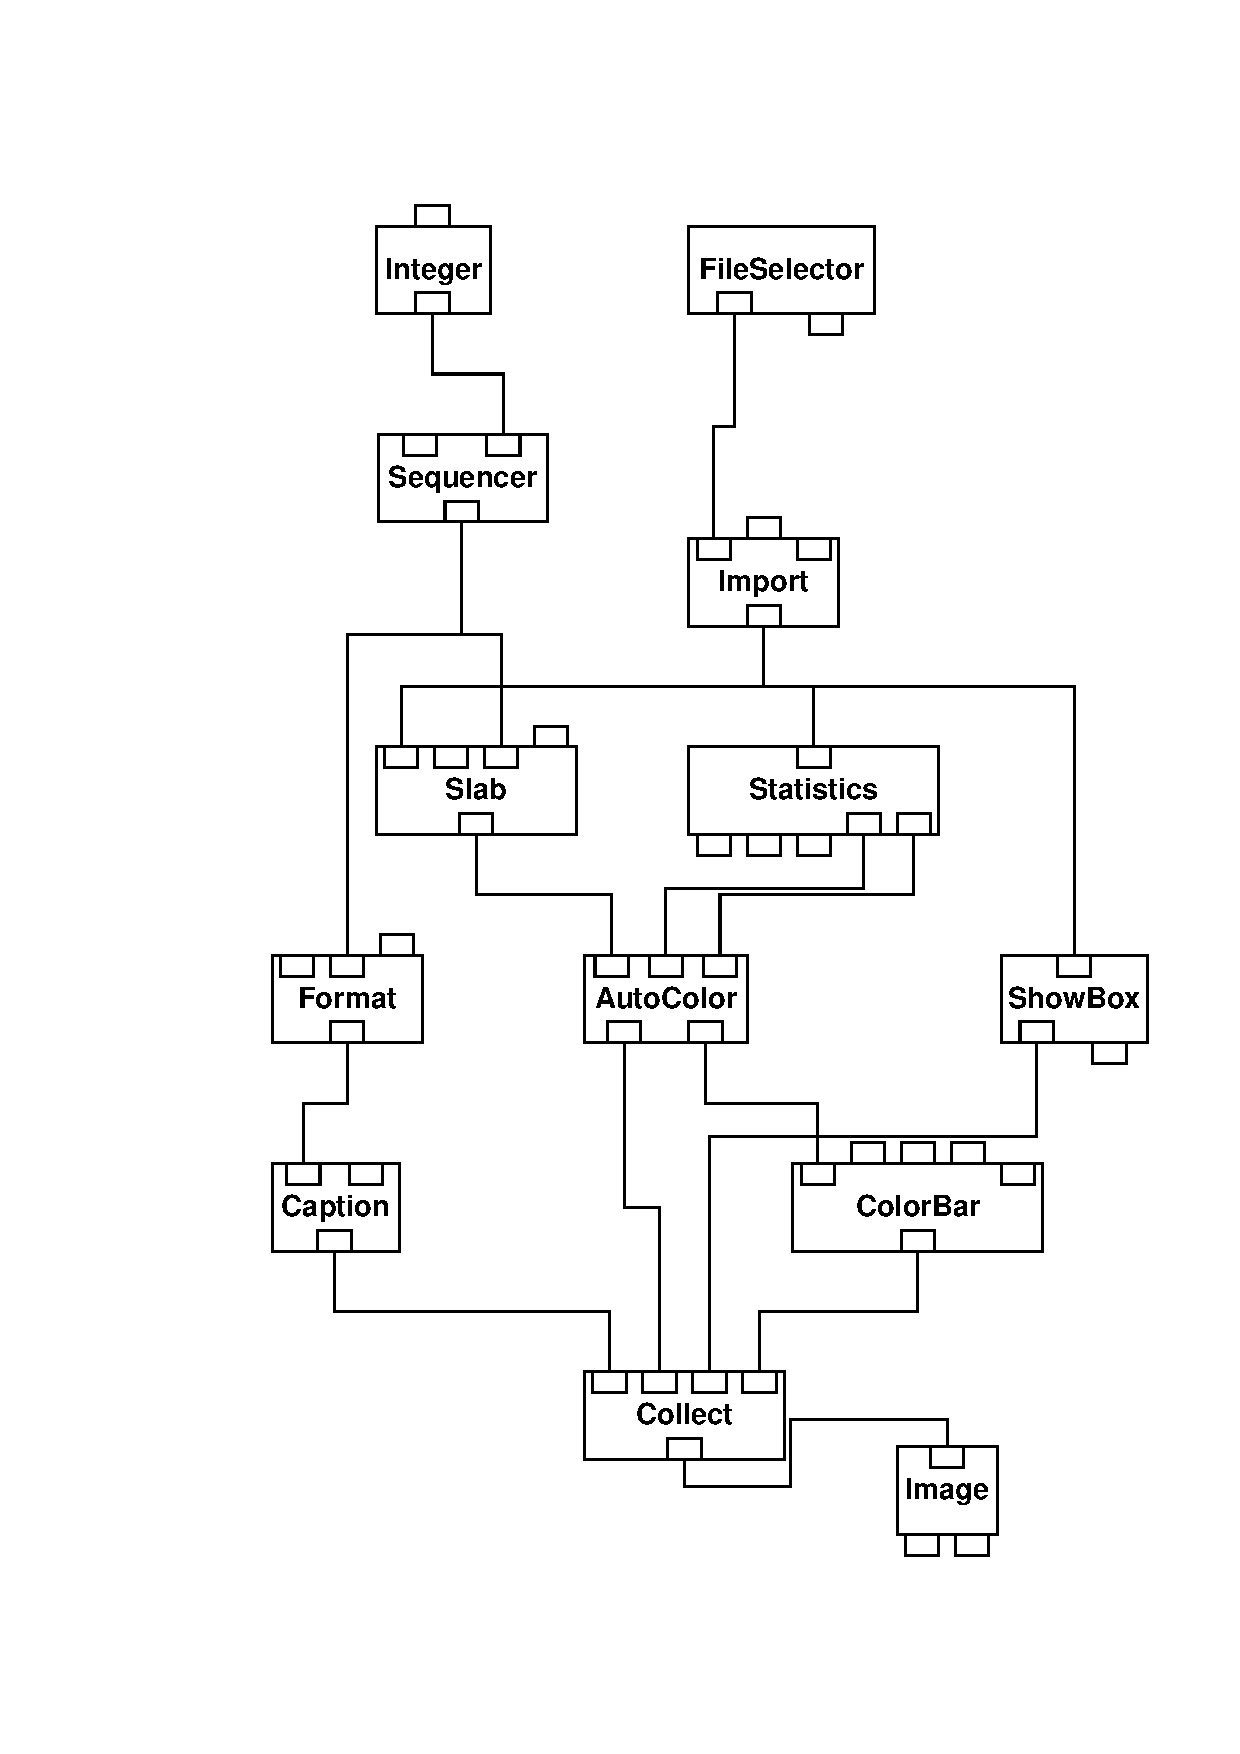
\includegraphics[width=450pt]{sc2_jcmtslice}
  \end{center}

  \caption[Network to display a sequence of slices through a JCMT
   data cube.]{Network to display a sequence of slices through a JCMT
   data cube. \label{JCMTSLICE} }

  \end{figure}

  \begin{enumerate}

    \item Load the network.  Select the `Open Program' option from the
     `File' menu of the main DX window.  Select file \texttt{jcmtslice.net}.  The network should now load and appear in the
     main window.  See Section~\ref{BASIC} for further details.

    \item Select the `Open All Control Panels' option from the `Windows'
     menu of the main DX window.  Set the required file name and
     number of slices.  (In the current example these are \texttt{l1689bsub.dx} and 20 respectively.)  Close the `Control Panel'
     window.

    \item Execute the network once.  Once the network has executed you
     will probably have to reset the display window (option `Reset' in
     the `Options' menu of the display window).  For a more effective
     display select `View control' from the `Options' menu and set the
     `Set View' parameter to one of the `Off' options, perhaps `Off top'.

    \item Finally double click on the `Sequencer' module and click on
     the play button.  A sequence of slices sweeping through the data
     cube will now be displayed.

  \end{enumerate}

   The network includes a `scale bar' showing how the colour displayed
   for each pixel in each slice corresponds to the value of the pixel.
   In this example the value of each pixel is the radio `brightness
   temperature' in kelvin.

  \item Figure~\ref{JCMTSURFACE} shows a network for displaying an
   iso-surface\footnote{An iso-surface is the analogue in
   three-dimensional gridded data of a single contour in two-dimensional
   gridded data. That is, it is a surface defined by some constant value
   of the dependent variable.} in a JCMT data cube.  This network is
   available as files \texttt{jcmtsurface.net} and \texttt{jcmtsurface.cfg}
   (again \texttt{jcmtsurface.net} is the basic network and \texttt{jcmtsurface.cfg} is a configuration file).

  \begin{figure}[htbp]

  \begin{center}
  \leavevmode
  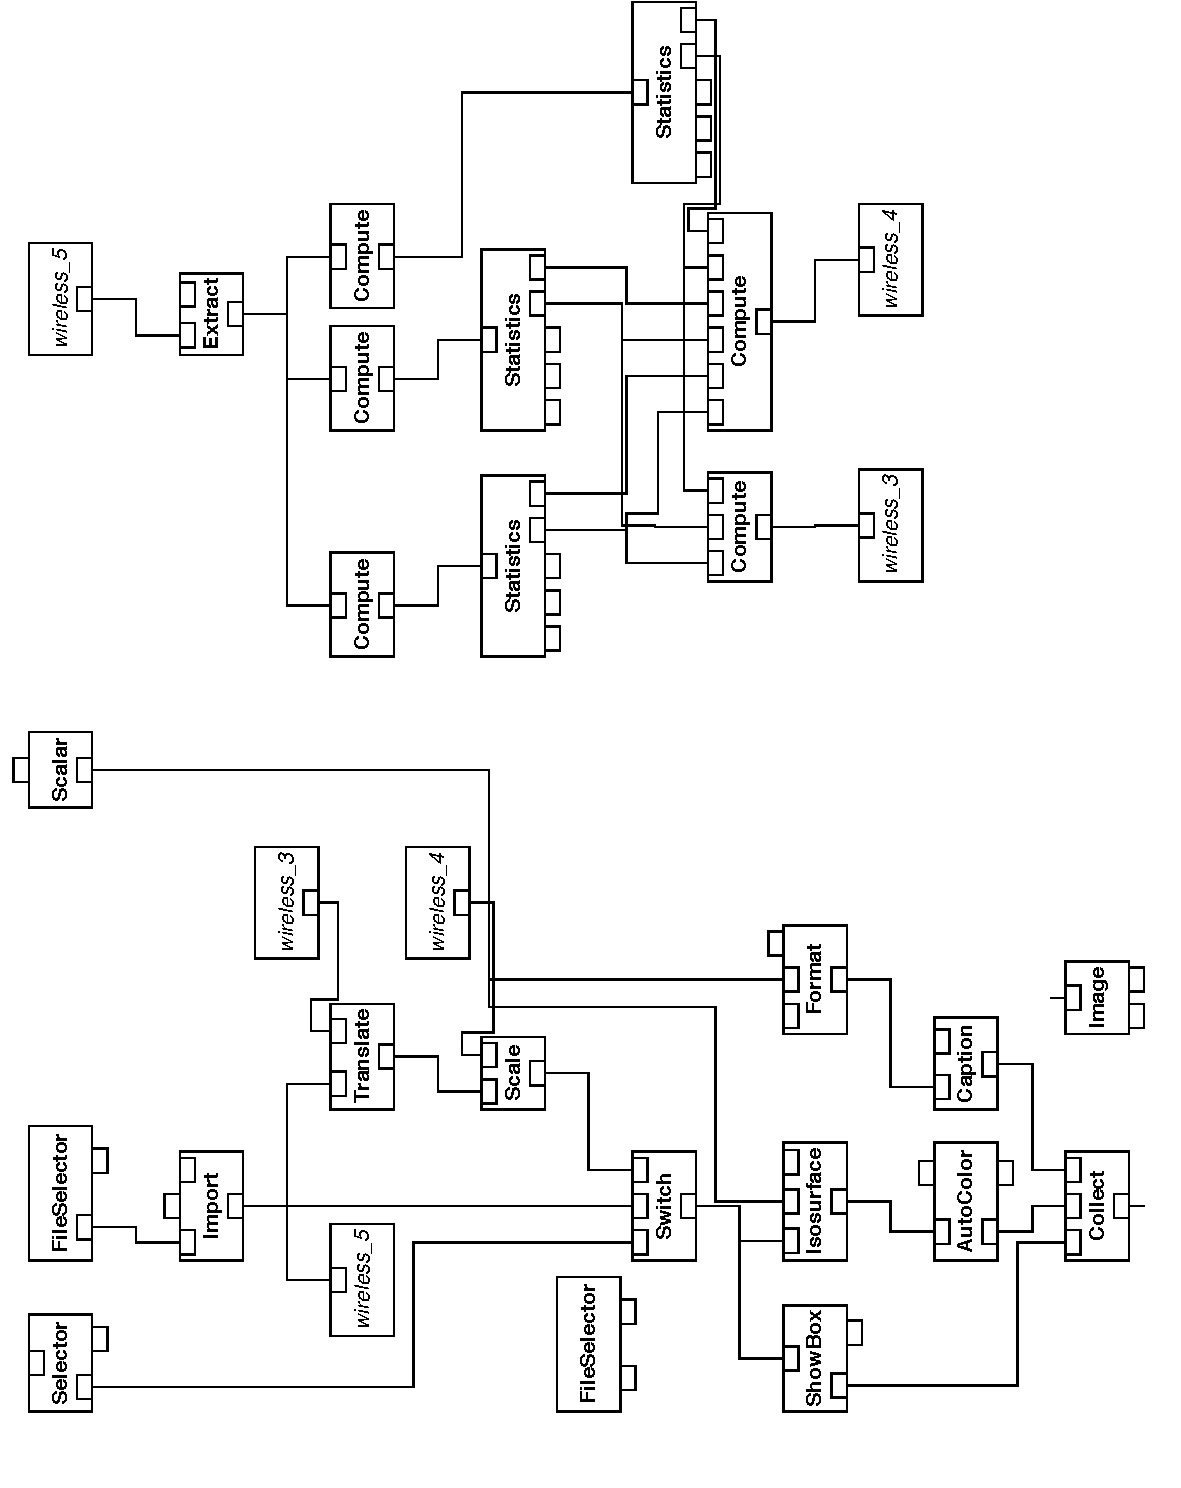
\includegraphics[height=450pt,angle=90]{sc2_jcmtsurface}
  \end{center}

  \caption[Network to display an iso-surface in a JCMT data cube.]
   {Network to display an iso-surface in a JCMT data cube.
   \label{JCMTSURFACE} }

  \end{figure}

   Much of the complexity of this network occurs because it contains an
   option to normalise the axes of the cube.  Two of the axes correspond
   to positions on the sky and the third to the dispersion, usually
   expressed as a radial velocity computed from the rest wavelength of
   the line.  There is no relation between the spacial and spectral
   axes, so the `cube' can be either very `long' or `thin' in the
   spectral axis compared to the spacial ones.  In order to generate
   an effective iso-surface it often helps to `normalise' the cube
   so that it has unit length in each axis.  Though this procedure
   often improves the iso-surfaces generated it makes the axes less
   intuitive.  Hence it is made optional so that you can choose the
   alternative most suitable for your data.

  \begin{enumerate}

    \item Select the `Open All Control Panels' option from the `Windows'
     menu of the main DX window.  Set the axis units, file name
     and iso-surface value.  In the current example suitable
     values of these quantities are: normalised, \texttt{l1689bsub.dx} and
     3.5 respectively.
     The contour (or iso-surface) value is specified as a radio
     `brightness temperature' in kelvin.  Close the `Control
     Panel' window.

    \item Execute the network once.  Once the network has executed you
     will probably have to reset the display window (option `Reset' in
     the `Options' menu of the display window).  For a more effective
     display select `View control' from the `Options' menu and set the
     `Set View' parameter to one of the `Off' options, perhaps `Off top'.
     Re-execute the network.

    \item Use the various settings of the `Mode' option in the `View
     Control' window to pan, zoom and rotate the display in order to
     examine the iso-surface.  These options are described in Section
     2.3 \textit{Controlling the Appearance of an Object: the Image
     Window}\, of the IBM \textit{QuickStart Guide}\cite{QUICKS}.

  \end{enumerate}

\end{enumerate}


\newpage
\section{\xlabel{ROSAT}\label{ROSAT}ROSAT Data Cube}

This recipe shows how to import and display a data cube observed with the
\htmladdnormallink{ROSAT}{http://heasarc.gsfc.nasa.gov/0/docs/rosat/rosat3.html}
X-ray astronomy satellite (\textit{R\"{o}ntgensatellit}).  ROSAT data come
in a number of different formats.  The example used here is an Asterix
binned dataset of the irregular galaxy M82 (NGC 3034).  This format is
used by the Asterix package (see \xref{SUN/98}{sun98}{}\cite{SUN98}).
The data cube comprises a grid of 216 by 216 points on the sky, with a
spectrum of 22 points at each position.  The example data are available
as file \texttt{m82ast.sdf}.  The procedure for importing and displaying these
data is very similar to the corresponding procedure for JCMT data
described in Section~\ref{JCMT}.

\begin{enumerate}

  \item The first stage to importing an Asterix binned dataset is to
   convert it to a simple data cube in the standard Starlink
   \xref{NDF}{sun33}{} format.  Application \texttt{ast2ndf} in the CONVERT
   package (see \xref{SUN/55}{sun55}{}\cite{SUN55}) performs this task.
   Proceed as follows.  First type:

\begin{terminalv}
% convert
\end{terminalv}

   to make the CONVERT applications available.  Then type:

\begin{terminalv}
% ast2ndf   m82ast  m82ndf
\end{terminalv}

   Note that though the input Asterix binned dataset and output NDF are
   respectively
   held in files called \texttt{m82ast.sdf} and \texttt{m82ndf.sdf} they are
   specified to application \texttt{ast2ndf} without the `\texttt{.sdf}' file
   type.

   It is also worth noting that an Asterix binned dataset is itself
   almost a standard Starlink NDF.  \texttt{ast2ndf} merely makes the
   data format completely standard and rearranges the order of the
   axes.

  \item Once the Asterix binned dataset has been converted to a simple
   data cube in the NDF format then a variety of standard Starlink
   applications can be used to process and display it.  For example, it
   can be accessed with the image processing applications in KAPPA (see
   \xref{SUN/95}{sun95}{}\cite{SUN95}).  It is also possible to inspect
   the structure of the data set using \texttt{hdstrace}.  Simply type:

\begin{terminalv}
% hdstrace  m82ndf
\end{terminalv}

   Again the file name is specified without the `\texttt{.sdf}' file type.
   This facility is useful because it lists the value of much of the
   auxiliary information contained in the data set.  \texttt{hdstrace}
   is documented in \xref{SUN/102}{sun102}{}\cite{SUN102}.  In addition,
   \texttt{hdstrace} and many other standard Starlink applications, will
   also work on the original Asterix binned dataset.

  \item The next step is to convert the NDF format file into a file
   in the `native' DX format, which DX can read.  This operation
   could be performed `on the fly' as DX reads the file.  However, it
   is simpler to convert the file in a separate operation prior to
   invoking DX.  The conversion is performed using application
   \xref{\texttt{ndf2dx}}{sun203}{NDF2DX}, which is part of SX, the
   Starlink enhancements to DX (see \xref{SUN/203}{sun203}{}\cite{SUN203}).
   By convention files in the native DX format have file type `\texttt{.dx}'.
   To convert the entire data cube simply type:

\begin{terminalv}
% $SX_DIR/ndf2dx  m82ndf  m82.dx
\end{terminalv}

   Note that though the file type is not specified for the input NDF
   file, it should be given for the output native DX format file.

   The above example will convert the entire data cube.  However, often
   the useful information will be contained in only a small range of
   energies.  For example, in the example dataset most of the
   useful information lies between energy steps 5 and 15.  It is
   possible to convert a subset of the NDF corresponding to a given
   range of energy steps.  For example, to convert a subset
   corresponding to steps 5 through to 15 type:

\begin{terminalv}
% $SX_DIR/ndf2dx  'm82ndf(5:15,,)'  m82sub.dx  axes=no
\end{terminalv}

   The syntax to specify a subset of an NDF is to give the bounds of
   the required region inside parentheses after the file name.
   Unfortunately however, by default the Unix shell will attempt to
   interpret these parentheses.  Thus, in the above example the input
   file name and NDF subset are enclosed in single quotes in order to
   prevent this behaviour and ensure they are passed correctly to \texttt{ndf2dx}.  The use of `escape mechanisms'  of this sort to prevent the
   premature interpretation of special characters sent to Starlink
   applications is discussed in \xref{SC/4}{sc4}{sc4_se_spec_char}\cite{SC4}.

   The \texttt{axes=no} option causes \texttt{ndf2dx} to ignore any axis
   information present in the input dataset and write the output DX file
   with axes consisting of simple pixel numbers.  This option may or
   may not be appropriate depending on the details of your data.
   In the present case it leads to a better visualisation.

  \item Figure~\ref{ROSATSLICE} shows a DX network to display a sequence
   of slices through a ROSAT data cube Each slice corresponds to the
   grid of points seen on the sky at a given radial velocity.  The network
   is available as files \texttt{rosatslice.net} and \texttt{rosatslice.cfg}
   (\texttt{rosatslice.net} is the basic network and \texttt{rosatslice.cfg} is
   a `configuration file' which controls some aspects of its behaviour).
   Start DX (as described in Section~\ref{START}).  Then proceed as
   follows.

  \begin{figure}[htbp]

  \begin{center}
  \leavevmode
  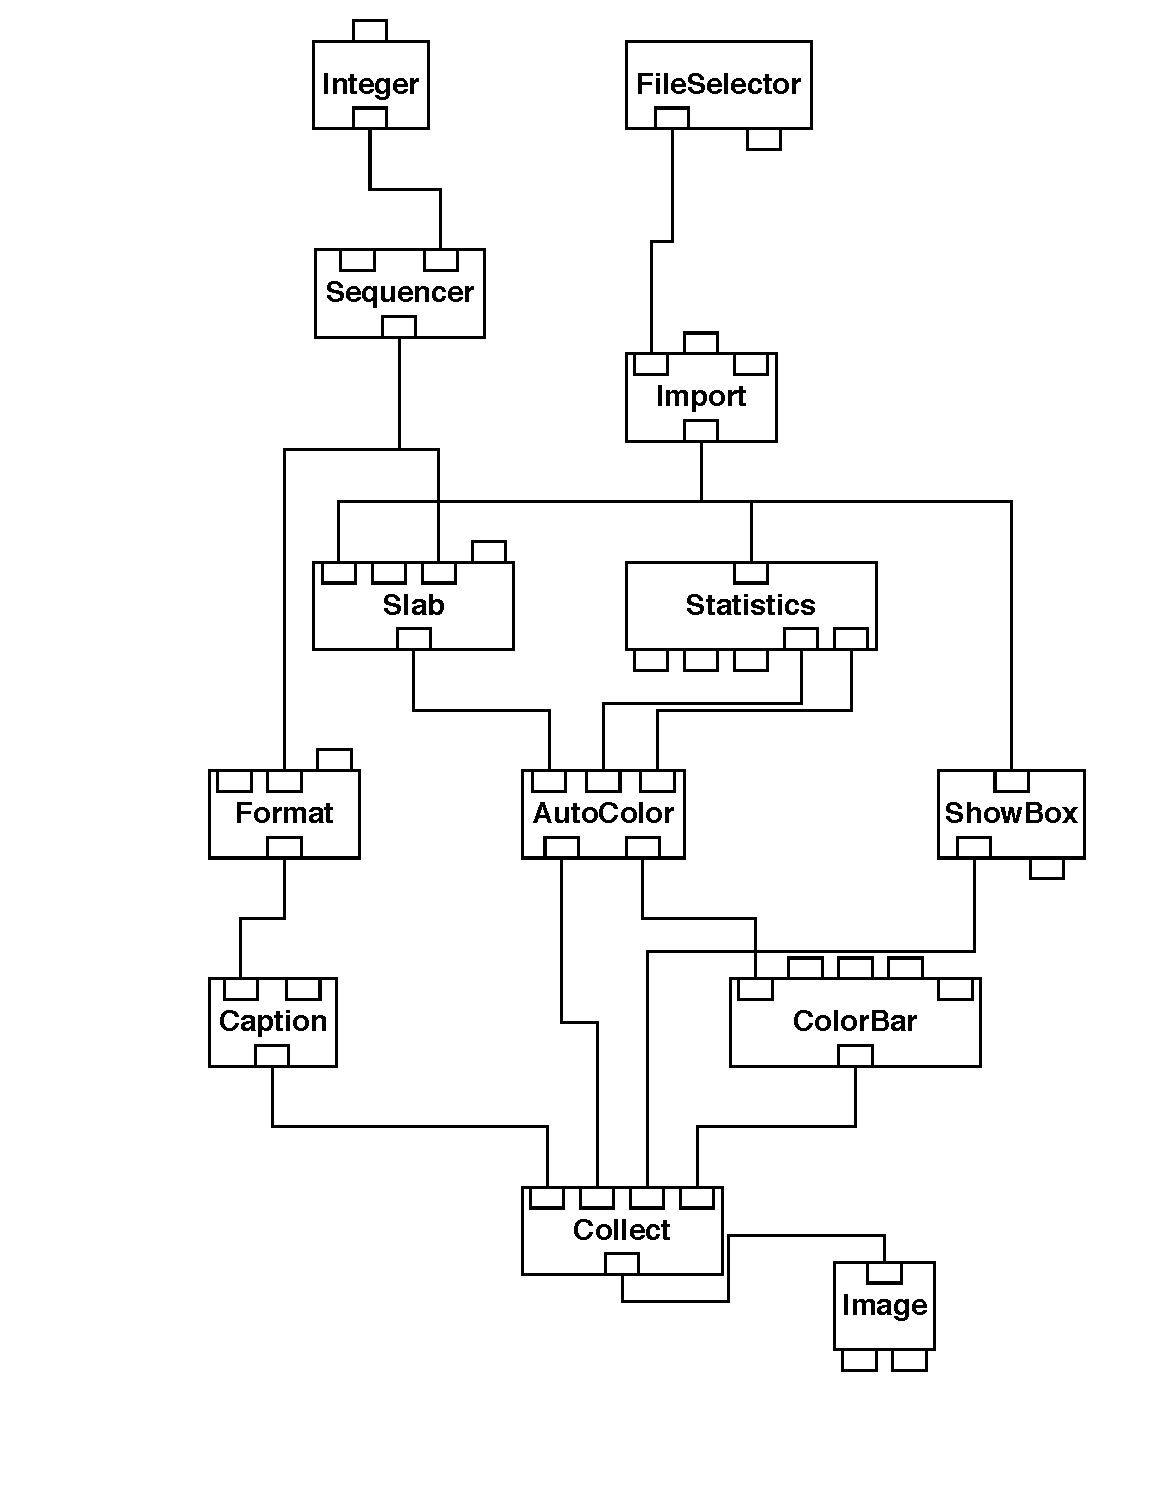
\includegraphics[width=450pt]{sc2_rosatslice}
  \end{center}

  \caption[Network to display a sequence of slices through a ROSAT
   data cube.]{Network to display a sequence of slices through a ROSAT
   data cube. \label{ROSATSLICE} }

  \end{figure}

  \begin{enumerate}

    \item Load the network.  Select the `Open Program' option from the
     `File' menu of the main DX window.  Select file \texttt{rosatslice.net}.  The network should now load and appear in the
     main window.  See Section~\ref{BASIC} for further details.

    \item Select the `Open All Control Panels' option from the `Windows'
     menu of the main DX window.  Set the required file name and
     number of slices.  (In the current example these are \texttt{m82sub.dx}
     and 10 respectively.)  Close the `Control Panel' window.

    \item Execute the network once.  Once the network has executed you
     will probably have to reset the display window (option `Reset' in
     the `Options' menu of the display window).  For a more effective
     display select `View control' from the `Options' menu and set the
     `Set View' parameter to one of the `Off' options, perhaps `Off top'.

    \item Finally double click on the `Sequencer' module and click on
     the play button.  A sequence of slices sweeping through the data
     cube will now be displayed.

  \end{enumerate}

   The network includes a `scale bar' showing how the colour displayed
   for each pixel in each slice corresponds to the value of the pixel.
   In this example the value of each pixel is the count rate in counts
   per second.  This network for displaying ROSAT data is virtually
   identical to the corresponding network for JCMT data (see
   Section~\ref{JCMT} and Figure~\ref{JCMTSLICE}).  The only differences
   are the defaults for the file names and the axis labels.  Similarly,
   the network for generating an iso-surface in JCMT data (see
   Figure~\ref{JCMTSURFACE}) requires only minor cosmetic modifications
   to display ROSAT data.

\end{enumerate}


% - Part III ----------------------------------------------------------
\cleardoublepage

\part{The DX Data Model}

\section{\xlabel{INTRO_DATMOD}Introduction}

DX has a powerful and flexible data model capable of representing many
sorts of data. Whilst you do not need to understand the data model in
detail, you will be able to use DX more effectively if you have a
rudimentary understanding of it. Section~\ref{BLUFFER} gives a very
brief summary of the data model. If you do not like reading manuals
it might just about give you enough information to get by.
Section~\ref{OUTLINE} presents a slightly longer, but still quite short,
introduction to the data model. I recommend that you read it if you are
planning to make a significant amount of use of DX.

\subsection{Further reading}

The DX data model is fully described in Chapter~2 \textit{Introduction
to Visualization}, especially Section 2.1, and Chapter~3 \textit{Understanding
the Data Model}\, of the IBM \textit{User's Guide}\cite{USERG}.


\section{\xlabel{BLUFFER}\label{BLUFFER}Summary}


In DX the basic entity used to represent a data cube or a particle (or
catalogue) dataset is called a \textbf{field} (this usage is similar to the
use of the term `field' in physics, for example, `velocity field', but
is different from the usual use in computing). Each field consists of a
set of \textbf{components}; arrays holding the \textbf{positions} of the data
points and a \textbf{data} array containing the dependent variable. The
data array may contain either scalar or vector data. For particle (or
catalogue) data, where the positions of the points are not related to
each other, the field need only contain the positions and data
components. However, for gridded data there is an additional \textbf{connections} array which defines the relation between neighbouring
points in the grid and controls how interpolation is performed.

In DX gridded data may be either position dependent or connection
dependent.

\begin{description}

  \item[Position dependent] The data array contains instantaneous
   samples of the underlying field computed at the position of each
   grid point.

  \item[Connection dependent] The grid points delineate the corners
   of a cell. The data array contains the value inside this cell.

\end{description}

The practical difference between the two cases is that for position
dependent data new values for positions intermediate between grid points
are interpolated, whereas for connection dependent data they are not
(the single data value applies to the entire cell). Position dependent
data are probably more common in astronomy.


\section{\xlabel{OUTLINE}\label{OUTLINE}Outline of the Data Model}


The data structures which can be represented using the DX data model
include:

\begin{enumerate}

  \item data defined on a regular orthogonal grid,

  \item data defined on a deformed regular or curvilinear grid,

  \item data defined on various sorts of irregular grids,

  \item unstructured data with no connection between the data points.

\end{enumerate}

In the first case the dependent variable (which is the quantity to be
visualised), perhaps for example, temperature, is sampled in a regular
grid inside some region defined with the independent variables as axes.
Usually the independent variables will be positions in two, three or
higher dimensions. Typically inside your own programs such data would be
represented as an array of appropriate dimensionality. The second and third
cases are generalisations of the first and can be ignored for our present
purposes. The fourth case corresponds to particle (or catalogue) data.
Here each point is simply a point in an assemblage or cloud of points;
there is no connection in terms of either the independent variables
(positions) or the dependent variable between the points. An example
might be a simulation of a globular cluster where each data point
corresponds to a separate star following its own orbit inside the
cluster.

Any of the four cases can occur with any dimensionality: one, two,
three and higher dimensional data can be represented. Similarly all
the usual data types are available: integer, real, double precision,
complex etc. The dependent quantity may be a scalar (such as temperature,
pressure or energy) or a vector (such as velocity or momentum).

The fundamental entity in the DX data model is an \textbf{object}. Data
are represented by the same set of objects both when they are resident
in memory when DX is running and when they are stored in native format
disk files\footnote{It is also, of course, possible to input files
written in a wide variety of other formats; see Sections~\ref{IMP_GRID}
and \ref{IMP_PART} for some examples.}. There are several sorts of objects.
For the present purposes the most important type of object is the \textbf{field}; usually each separate dataset will be represented as a single
field\footnote{This usage of the term `field' corresponds to its usual
meaning in physics rather than in computing. For example, a DX field may
represent a three-dimensional grid holding a set of samples of the
velocity field throughout some volume. This usage is quite different from
the usual meaning in computing: a predetermined section of a record
allocated to the storage of a particular data item. Anyone used to the
computing terminology should particularly beware of this different
usage.}.

A field consists of an arbitrary number of \textbf{components} and each
component itself has a number of \textbf{attributes}. This hierarchy is
illustrated in Figure~\ref{DXITEMS}.

\begin{figure}[htbp]

\begin{center}

\begin{tabular}{l}
\texttt{field     } \\
\texttt{~~component 1   } \\
\texttt{~~~~attribute 1 } \\
\texttt{~~~~attribute 2 } \\
\texttt{~~~~~~~~~.      } \\
\texttt{~~~~~~~~~.      } \\
    \\
\texttt{~~component 2   } \\
\texttt{~~~~attribute 1 } \\
\texttt{~~~~attribute 2 } \\
\texttt{~~~~~~~~~.      } \\
\texttt{~~~~~~~~~.      } \\
   \\
\texttt{~~component 3   } \\
\texttt{~~~~~~~.        } \\
\texttt{~~~~~~~.        } \\
\end{tabular}
\end{center}

\begin{quote}
\caption[The hierarchy of items in a DX field.]{The hierarchy of items in
a DX field. Indenting to the right indicates successively lower levels in
the hierarchy. \label{DXITEMS} }
\end{quote}

\end{figure}

\subsection{Components}

There are many different types of component. Some are mandatory, but
most are optional. Only a few of the more common ones are relevant to
the present discussion. They are listed in Table~\ref{COMPONENTS} and
described below.

\begin{table}[htbp]

\begin{center}
\begin{tabular}{rcl}
Name        & Mandatory? & Comments                                \\ \hline
positions   & $\bullet$  & position of each datum                  \\
data        & $\bullet$  & value of each datum                     \\
connections &            & relation between data points            \\
box         &            & bounding box for positions in the field \\
\end{tabular}
\end{center}

\begin{quote}
\item \caption[Common components of a field.]{Common components of a field.
\label{COMPONENTS} }
\end{quote}

\end{table}

\begin{description}

  \item[Positions] The position component is an array\footnote{Strictly
   speaking this array, and other arrays in components, are themselves
   DX objects of type \textbf{array}. However, this complication is not
   important to the present discussion and it is adequate to think of
   the component as simply an array of numbers.} defining a
   position for every datum in the dataset. If the field contains
   unconnected particle data then the array will be a simple list
   with a position for each datum. If the field contains a regular
   grid the positions can be represented more compactly as a \textbf{regular} or \textbf{product} array; essentially just the origin, size
   and increment of the grid are stored.

  \item[Data] The data component is an array storing the dependent
   variable: temperature, density, velocity, momentum or whatever.

  \item[Connections] The connections component prescribes to DX how
   to perform interpolation between neighbouring grid elements. It
   is described further in Section~\ref{CONINT}, below. In unstructured
   particle or catalogue data the connection component is absent
   (because the position of one particle bears no relation to the
   position of any other particle; think of the example of stars following
   their individual orbits within a globular cluster).

  \item[Box] The box component is an array of $2^{n}$\, points where
   $n$\, is the dimensionality of the positions component. The values
   contain the coordinates of a bounding box sufficiently large to
   just enclose all the positions of a field.

\end{description}

\subsection{Attributes}

Components can have \textbf{attributes} associated with them. Attributes
are additional items of information describing some aspect of the
component. For example, the dependency attribute, `dep', identifies
another component on which the component depends; the `data' component
may depend on either the positions or the connections component, depending
on circumstances. Alternatively the component `ref' indicates that a
component refers to another component. Typically the connections
component will have a `ref' of `positions', indicating that the
connections refer to the positions.

\subsection{\label{CONINT}The connections component and interpolation}


The connections component prescribes to DX how to perform interpolation
between neighbouring grid elements. It describes the logical
connectivity between adjacent neighbours in a grid. For example, the
interpolation could be performed linearly along one of the axes, or
bi- or tri-linearly along two or more axes simultaneously.

The connections component is implemented as an array. Each point in the
positions component is given an ordinal number (starting at zero). The
connections array comprises a `list of lists' of numbers in which each
entry represents the ordinal values of the points that are to be
connected, listed in the order that they are to be connected.

You will not normally need to be concerned with the full details of the
connections component. For a regular grid it can be created
automatically when the data are imported into DX and represented
compactly using a \textbf{path} or \textbf{mesh} array.

Fields representing particle or catalogue data where there are no
logical connections between elements in the positions component will
not usually have a connections component (again think of the example
where each point represents a star orbiting in a globular cluster).

\subsection{\label{POSCONDEP}Position and connection dependent data}


For a field of gridded data (it is easier to think of a regular grid,
though the argument applies equally to an irregular grid) there are two
ways in which the dependent variable can relate to the elements of the
grid.

\begin{description}

  \item[Position dependent] The dependent variable represents
   instantaneous samples of the underlying field (temperature, pressure,
   momentum or whatever), computed at the position of each grid point.

  \item[Connection dependent] The grid points delineate the corners
   of a cell. The dependent variable is the value inside this cell.
   An example might be a grid spanning a globular cluster with the
   dependent variable being the number of stars in each cell.

\end{description}

The practical difference between the two cases is the way in which
values for the dependent variable are computed at positions intermediate
between grid points.

\begin{description}

  \item[Position dependent] A value for the dependent variable is
   interpolated from its values at the neighbouring grid points.

  \item[Connection dependent] The value of the dependent variable for
   the cell is used for any positions inside the cell (because the
   value pertains to the entire cell, not just one instantaneous
   point).

\end{description}

The dependency attribute, `dep', of the data component will be set to
`positions' if the data are position dependent and to `connections' if
they are connection dependent.

Before you input data to DX you must decide whether they are position
dependent or connection dependent. Position dependent data are probably
more common in astronomy.


\newpage
\section{\xlabel{ACK}\label{ACK}Acknowledgements}

Derek~Ward-Thompson and Nick~Jessop kindly provided the JCMT SPECX map and
Dave~Strickland the ROSAT Asterix binned dataset.  David~Berry gave much
useful advice and assistance with DX and suggested several improvements to
a draft version of the document.


\addcontentsline{toc}{section}{References}
\begin{thebibliography}{99}

  \item[~] The references are listed alphabetically by title.  In the
   case of Starlink documents the document code (for example SC/4.1
   or SUN/17.6) forms part of the title.

  \bibitem{QUICKS} \textit{IBM Visualization Data Explorer: QuickStart
   Guide}, Second Edition, 1995, document reference number:
   SC34-3262-01.

  \bibitem{USERG} \textit{IBM Visualization Data Explorer: User's Guide},
   Sixth Edition, 1995, document reference number: SC38-0496-05.

  \bibitem{SC4} \xref{SC/4.1}{sc4}{}:
   \textit{C-shell Cookbook}\, by M.J.~Currie, 2 May 1997 (Starlink).

  \bibitem{SG8} \xref{SG/8.2}{sg8}{}:
   \textit{An Introduction to Visualisation Software for Astronomy}\,
   by A.C.~Davenhall, 4 March 1997 (Starlink).

  \bibitem{SUN17} \xref{SUN/17.6}{sun17}{}:
   \textit{SPECX -- A Millimetre Wave Spectral Reduction Package}\, by
   R.M.~Prestage, H.~Meyerdierks and    J.F.~Lightfoot, 13 January 1995
   (Starlink).

  \bibitem{SUN55} \xref{SUN/55.6}{sun55}{}:
   \textit{CONVERT -- A Format-conversion Package}\, by M.J.~Currie,
   G.J.~Privett and A.J.~Chipperfield, 7 December 1995 (Starlink).

  \bibitem{SUN86} \xref{SUN/86.12}{sun86}{}:
   \textit{FIGARO -- A General Data Reduction System}\, by K.~Shortridge,
   H.~Meyerdierks, M.J.~Currie and M.J.~Clayton, 26 September 1996
   (Starlink).

  \bibitem{SUN95} \xref{SUN/95.9}{sun95}{}:
   \textit{KAPPA -- Kernel Application Package}\, by M.J.~Currie,
   9 December 1995 (Starlink).

  \bibitem{SUN98} \xref{SUN/98.6}{sun98}{}:
   \textit{ASTERIX -- X-ray Data Processing System}\,
   D.J.~Allan and R.J.~Vallance, 13 May 1995 (Starlink).

  \bibitem{SUN102} \xref{SUN/102.3}{sun102}{}:
   \textit{HDSTRACE -- Listing HDS Data Files}\, by M.J.~Currie,
   14 February 1994 (Starlink).

  \bibitem{SUN203} \xref{SUN/203.3}{sun203}{}:
   \textit{DX -- IBM Data Explorer for Data Visualisation}\, by D.S.~Berry,
   G.J.~Privett and A.C.~Davenhall, 15 September 1997 (Starlink).

\end{thebibliography}


\typeout{  }
\typeout{*****************************************************}
\typeout{  }
\typeout{Reminder: run this document through Latex twice}
\typeout{to resolve the references.}
\typeout{  }
\typeout{*****************************************************}
\typeout{  }

\end{document}
